\documentclass[a4paper, 11pt]{article}
\usepackage[top=3cm, bottom=3cm, left = 2cm, right = 2cm]{geometry} 
\geometry{a4paper} 
\usepackage[utf8]{inputenc}
\usepackage{textcomp}
\usepackage{graphicx} 
\usepackage{amsmath,amssymb}  
\usepackage{bm}
\usepackage[pdftex,bookmarks,colorlinks,breaklinks]{hyperref}  
\hypersetup{linkcolor=black,citecolor=black,filecolor=black,urlcolor=black} % black links, for printed output
\usepackage{memhfixc} 
\usepackage{pdfsync}  
\usepackage{fancyhdr}
\usepackage{pdfpages}
\usepackage{tabularx}
\usepackage{multirow}
\usepackage{colortbl}
\usepackage{float,graphicx}




\pagestyle{fancy}

\renewcommand\tabularxcolumn[1]{m{#1}}

\title{GIS Hydrography Management System for Provincial Waters}
\author{Boscolo Cegion Nicola}
\author{Cazzaro Mirco, Boscolo Cegion Nicola}
\date{}
\begin{document}



\begin{center}
	\begin{minipage}{2.5cm}
	\begin{center}
		
\includegraphics[height=1.8cm]{img/unipd.png}
		
	\end{center}
\end{minipage}\hfill
\begin{minipage}{10cm}
	\begin{center}
	\textbf{Uneversity of Padua}\\[0.1cm]
    \textbf{Computer Engineering}\\[0.1cm]
    \textbf{Geographic Information Systems}


	\end{center}
\end{minipage}\hfill
\begin{minipage}{2.5cm}
	\begin{center}
		
\includegraphics[height=2.5cm]{img/belluno.png}
	\end{center}

\end{minipage}



\textsc{\Large }\\[1.5cm]
{\large \bfseries Exam project}\\[4.5cm]


{\huge \bfseries \uppercase{GIS Hydrography Management System for Provincial Waters} \\[0.5cm] }
\textsc{\Large }\\[2.5cm]







\begin{tabular}{c}
    Made by:\\[0.5cm]
    {\LARGE Boscolo Cegion Nicola}\\[0.1cm]
    {\LARGE Cazzaro Mirco}\\[0.1cm]
    
\end{tabular}
\vfill

% Bottom of the page
{\textbf{\large {Academic Year} 2022-2023}}

\end{center}


\pagebreak
\tableofcontents

\section{Objective of the Studies}
\label{sec:objectives}

The objective of this project is to develop an information system for hydrography management in the Italian province of Belluno. The system aims to achieve the following goals:
\begin{itemize}
    \item Know the situation of all the water resources in the province: The system will provide comprehensive information about the water bodies within the province, including lakes and rivers. It will facilitate the understanding of the current state of these water resources.
    \item Manage inputs of potentially polluting liquids: The system will enable the management and monitoring of inputs that have the potential to pollute the water resources. It will track and control the release of substances into the water bodies to ensure environmental protection.
    \item Monitor the status of provincial waters: The system will continuously monitor and gather data on the condition of water resources, including parameters like water level, flow, turbidity, temperature, pH, dissolved oxygen, and more. It will enable the province to assess water quality and identify any anomalies or pollution incidents promptly.
    \item Compliance with European standards: The system will adhere to the relevant European standards for the representation of water networks. It will ensure that the information system follows the prescribed guidelines and formats for accurate and standardized data representation.
\end{itemize}

By achieving these objectives, the hydrography management system will provide the province with an efficient tool to monitor, manage, and protect its water resources effectively.


\section{Analysis of Requirements}
\label{sec:requirements}

\subsection{Functional Requirements}
\begin{itemize}
    \item \textbf{Import and Export of Data}: The system must support the seamless import and export of data in various standard formats, including shape files. This capability will enable data integration from diverse sources and facilitate interoperability with other systems.
    \item \textbf{Network Update}: The system should allow authorized personnel to update both the geometric and attribute aspects of the water network. It must ensure data consistency by maintaining a comprehensive history of modifications, enabling traceability and analysis of network changes over time.
    \item \textbf{Query System}: A robust interrogation system is necessary, equipped with spatial and alphanumeric filters that can be combined. This will empower users to perform complex queries, extracting relevant information based on specific criteria for data retrieval and analysis.
    \item \textbf{Query Results Export}: Users should have the ability to export query results in compatible formats for further analysis, reporting, or integration with external tools and systems. This functionality enhances data utilization and supports informed decision-making processes.
    \item \textbf{Cartography and Orthophoto Visualization}: The system should provide an intuitive visualization interface, allowing users to overlay cartographic and orthophoto data as a background for analysis purposes. This feature enables the correlation of additional information with spatial context, aiding in decision-making.
\end{itemize}

\subsection{Data Requirements}
The system necessitates the following data (with the following charateristics) to fulfill its objectives in the hydrography management system:
\begin{itemize}
    \item \textbf{Required Data}: Comprehensive information regarding water bodies within the province, including spatial attributes (geometry), essential attributes (e.g., name, type), and historical records of network modifications.
    \item \textbf{Data Format}: The system should support multiple data formats for efficient data management and interoperability. Primarily, the system should be capable of working with shape files, which are widely used in the geospatial domain. Shape files provide a standard format for storing both the geometry and attributes of geographic features. This format ensures compatibility with existing datasets and enables seamless integration with other geospatial systems.
                                Furthermore, the system should support commonly used formats for import and export operations, such as CSV (Comma-Separated Values) and GeoJSON (a format for encoding geospatial data in JSON). These formats facilitate data exchange with external systems and enable data analysis using various tools and applications.
                                By accommodating these diverse data formats, the system can effectively handle the information related to the water bodies, ensuring compatibility with existing data sources and promoting data interoperability within the hydrography management domain.
\end{itemize}


\subsection{Nonfunctional Requirements}
To ensure the development of an effective hydrography management system, the following nonfunctional requirements must be considered:
\begin{itemize}
    \item \textbf{Use of PostgreSQL DBMS}: The system should leverage the PostgreSQL database management system (DBMS) for efficient data storage, retrieval, and management. The utilization of this reliable and widely adopted DBMS will contribute to the system's scalability and performance. Within PostgreSQL, a powerful plugin for it called PostGIS will be used, so to expand the DBMS capabilities on managing spatial data.
    \item \textbf{Use of FOSS Components}: The system should embrace the use of Free and Open Source Software (FOSS) components during its development. By leveraging FOSS tools and libraries, the system can benefit from community support, cost-effectiveness, and flexibility in customization.
    \item \textbf{Compliance with Applicable Standards}: The system must adhere to applicable national and international standards for hydrography management and data representation. This compliance ensures interoperability, facilitates data sharing, and promotes compatibility with other systems within the domain.
    \item \textbf{Compliance with Rules and Regulations}: The system should conform to all relevant rules and regulations governing water management and environmental protection at both national and international levels. Adherence to these regulations ensures legal compliance and promotes responsible data handling practices.
\end{itemize}


\section{Starting Situation}
\label{sec:starting_situation}

In order to provide a comprehensive understanding of the project context, it is important to analyze the starting situation, including the existing technology, available data, and market analysis.

\subsection{Technology} The Province of Belluno currently operates an IT sector responsible for managing their Management Information System (MIS) using commercial software and the PostgreSQL database management system (DBMS). 
                        
                        However, a specific Geographic Information System (GIS) application tailored for hydrography management is not currently in place: our task is to develop a customized GIS solution to address this gap and fulfill the province's requirements.

\subsection{Exsisting Data} The region Veneto already possesses a topographic database built in accordance with the Italian national standard at the NC5 level. This database provides detailed information about the province's terrain and water features. The data is stored in the ETRF2000 reference system and can be accessed through OGC WMS (Web Map Service) and WFS (Web Feature Service) non-transactional services. 
                            
Additionally, orthophotos at a scale of 1:5000, also based on the ETRF2000 reference system, are available for visualization through WMS.

\subsection{Market Analysis} Extensive research indicates that there are currently no off-the-shelf or packaged solutions available in the market that adequately address the requirements of the hydrography management system for the Province of Belluno. 

                            This market gap presents an exciting opportunity for our team to develop a tailored solution that precisely meets the province's needs. By creating a custom application, we can ensure the fulfillment of all functional and nonfunctional requirements while complying with the relevant standards and regulations governing water resource management.

\subsection{Conclusions} Analyzing the starting situation in terms of existing technology, available data, and market conditions, it is evident that the development of a dedicated hydrography management system is crucial to effectively manage the province's water resources and address the current market gap.
\section{Working Hypotesis}
\label{sec:working_hypotesis}

The working hypothesis for this hydrography management project is based on careful analysis of the requirements and constraints. It forms the foundation for our approach and solution design. The following aspects outline our working hypothesis:

\subsection{Considerations}
Our primary focus is to develop a robust and scalable hydrography management system that effectively meets the needs of the Province of Belluno. We understand the importance of adhering to relevant standards and applying best practices in hydrography management. Additionally, we recognize the significance of user accessibility and aim to design the system as a web application, compatible with commonly used browsers such as Explorer, Chrome, and Firefox. We will also incorporate functionalities for specific use cases that may require customization using desktop GIS tools.

\subsection{Hypotesis}
Our hypothesis is that by implementing a customized GIS web application, integrated with a PostgreSQL DBMS, we can create an efficient hydrography management system that meets the specified requirements. The system will enable the province to document water bodies, manage intakes, monitor water conditions, perform data consultations, and handle citizen alerts effectively. To achieve this, the system will incorporate the following key features:
\begin{enumerate}
    \item Import and export of data in shape format and other standard formats to facilitate seamless integration with existing data sources and enable data exchange with external systems;
    \item Capability to update the network, both in terms of geometric elements and attribute data, while ensuring the historicization of changes. This will provide a comprehensive view of the network's evolution over time;
    \item An advanced interrogation system that combines spatial and alphanumeric filters to enable users to perform complex queries. This functionality will allow users to retrieve specific information based on their criteria;
    \item Export of query results to allow users to save and utilize the obtained data for further analysis or reporting purposes;
    \item Visualization of cartography and orthophotos as a background to enhance the analysis and interpretation of data within the system.
\end{enumerate}

In addition to these core features, the system will address specific requirements within the hydrography management domain. It will enable the province to:
\begin{enumerate}
    \item Manage intakes effectively by providing information on intake positions and attributes, facilitating the insertion and removal of intakes, and determining the route of pollutants released from intakes;
    \item Monitor water conditions by collecting real-time data from water monitoring units strategically placed across the province's waterways and lakes. The system will capture parameters such as level, speed, flow, turbidity, temperature, conductivity, pH, redox potential, dissolved oxygen, \textit{NH4+}, and \textit{CL-};
    \item Support maintenance activities for the control units, generating schedules for periodic maintenance and recording execution details to ensure the continuous and accurate functioning of the monitoring units;
    \item Enable data consultation by providing technical offices with the ability to perform combined searches based on spatial and attribute filters, as well as historical queries. The system will support complex queries such as identifying intakes in specific stretches of rivers or monitoring units measuring pH values below 6 within specific time intervals;
    \item Handle citizen alerts and facilitate transparent governance by creating a dedicated portal for daily publication of water quality analysis results. The system will include a reporting mechanism for citizens to anonymously report the presence of pollutants in the water, attaching photos and indicating the geographical location. Automatic filtering and relevance scoring of reports will be performed to reduce manual processing. The system will associate each alert with relevant monitoring units and previous alerts within a certain proximity.
\end{enumerate}

\subsection{Analysis of Risks and Constraints}
We will conduct a thorough analysis of potential risks and constraints that may affect the project's success. These could include technical challenges, data quality issues, resource limitations, and compliance requirements. We will develop mitigation strategies and contingency plans to address these risks and ensure smooth project execution.


\section{Preliminary Project}
\label{sec:preliminary_project}
The preliminary project section provides an overview of the hydrography management system project for the Province of Belluno. It covers various aspects, including goals, system functions, databases, technological components, project guidelines, operational aspects, risk management, benefits evaluation, and cost evaluation. This section serves as a comprehensive summary of the project, outlining its objectives, system functionalities, database structure, technical components, implementation guidelines, and assessment of potential benefits and costs. It provides a holistic view of the project's scope and sets the foundation for its successful execution and management.

\subsection{Goals}
The goals of the hydrography management system project for the Province of Belluno are defined to ensure the successful development, implementation, and utilization of the system. These goals provide a clear direction for our project team and serve as measurable outcomes to evaluate the project's success. The goals can be categorized into two key areas: overarching goals and intermediate goals.
\subsubsection{Overarching Goals}

\begin{itemize}
    \item \textbf{Develop a comprehensive hydrography management system}: The primary goal of the project is to design, develop, and implement a comprehensive hydrography management system tailored to the specific requirements of the Province of Belluno. The system will enable efficient management of water resources, including the documentation of water bodies, tracking of intakes, monitoring of water conditions, and citizen alert management;
    \item \textbf{Ensure user-friendly access and compatibility}: The system should provide a user-friendly interface accessible through popular web browsers such as Explorer, Chrome, and Firefox. Additionally, it should support specific functionality through customized desktop GIS tools when necessary. Compatibility and ease of use are essential to ensure widespread adoption and efficient utilization by technical offices, internal technicians, and citizens;
    \item \textbf{Adhere to relevant standards and regulations}: The system must comply with applicable hydrography management standards and regulations. It should ensure accurate data representation, support data interchangeability using standard formats, and promote interoperability with other systems in the hydrography management domain.
\end{itemize}

\subsubsection{Intermediate Goals}
\begin{itemize}
    \item Enable efficient data management, so to develop functionality for importing and exporting data in shape format and other standard formats, allowing seamless integration with existing datasets and data exchange with external systems. Implement mechanisms for network updates, both in terms of geometric elements and attribute data, ensuring the historicization of changes to track the evolution of the hydrography network;
    \item Implement advanced querying and visualization capabilities, so to create an advanced interrogation system that combines spatial and alphanumeric filters, empowering users to perform complex queries for retrieving relevant information. Enable the export of query results and provide visualization capabilities for cartography and orthophotos as a background, enhancing data analysis and decision-making processes;
    \item Support intake management, so to develop features to enable the identification and management of intakes, including their positions and attributes. Implement functionality for inserting new intakes, removing abandoned ones, and determining the routes of pollutants released from intakes;
    \item Facilitate water condition monitoring, so to design and implement mechanisms to collect real-time data from water monitoring units strategically located throughout the province. Capture key parameters such as water level, flow, turbidity, temperature, conductivity, pH, redox potential, dissolved oxygen, NH4+, and CL- to enable effective monitoring of water conditions;
    \item Enable maintenance planning and execution, so to develop functionality to support the scheduling and execution recording of periodic maintenance tasks for the monitoring units. Ensure timely and efficient maintenance to maintain accurate and reliable data collection;
    \item Enable data consultation and emergency detection, so to implement features that allow technical offices to carry out combined searches, spatial and attribute-based, as well as historical queries to retrieve relevant data. Develop mechanisms to detect and notify relevant personnel of potential emergencies through email notifications triggered by abnormal parameter values;
    \item Establish citizen reporting and transparency. The aim is to create a dedicated portal to publish daily water quality analysis results and promote transparent governance. Develop a reporting system for citizens to anonymously report pollutants with photo attachments and geographical location indications. Implement automatic filtering and relevance scoring of reports to streamline manual processing and associate alerts with relevant monitoring units and previous alerts.
\end{itemize}


\subsection{Technological Components}
Whenever talking about a system in the IT field it is implicit that different technological components (being them more or less interconnected) are required. In the case of the proposal for a Hydrography Management System, meeting the requirements of the customer, two different systems has top be developed: a desktop GIS system and a web GIS system, that are introduced in the following subsections and deeply explored in a dedicated paragraph. After that, software and hardware requirements need to be exploited.

\subsubsection{Database}
We can consider the database of the system the glue of all the other technological components. Furthermore, the customer already has in his IT sector a PostgreSQL database, that adapts perfectly to the system we want to develop, thanks to his extension \textit{PostGIS} that is suitable for managing spatial ang geographical data. Hence, this component will be used as the base for the developing of our application.
\subsubsection{Desktop GIS System}
Since is accepted that some of the functional requirements can be met through a desktop GIS application, and to stay adherent to the non-functional requirement of using FOSS components, the solution found is to develop specific plugins for the \textit{OpenJUMP} desktop application, making use of the \textit{Java™ JTS library}; the plugins built for the system will be packed together with the application and delivered to the customer. Technical support for the installation of the desktop system on customer terminals will be provided.
\subsubsection{Web GIS System}
The core of the system will be the web application: since it has to deliver to the user GIS capabilities, many components need to be integrated:
\begin{itemize}
    \item Frontend map management: it is necessary to provide to the users the possibility to use maps through the web app. For this, the OpenLayer JavaScript plugin will be used;
    \item Background map: it is necessary to display in this plugin a background map of the province: to meet this requirement, OpenStreetMap maps will be used;
    \item Backend spatial data delivery: it is necessary to deliver to the user (and to display over the OpenStreetMap) the spatial data that the Veneto Region has at disposal: for this, a dedicated Geoserver instance is necessary;
    \item Frontend implementation: parts of the web application shall be used also from the provincial citizens even on the go from mobile devices. In an optic of usability of the system with any device it is necessary of a full responsiveness of the system over any kind of terminal (smartphones, tablets, etc.) and to better integrate with other public IT systems, the \textit{Bootstrap Italia} template is our implementational choice.
\end{itemize}

\subsubsection{Hardware Requirements}
To support the functioning of the web application also from the exterior of the provincial organization, because of the active citizenship policy, but also to facilitate eventual and future possibilities of smart working activities of the provincial employees, a concrete possibility is the one of setting up a virtual private server hosted on the cloud: this possibility can be delivered both from a private hosting company, with a cost that has to be kept in consideration, or by the availability of some italian server infrastructure, if any.
The fact that the customer already owns a PostgreSQL database in their servers, can suggest to use them as hosting machines also for the system, but this can led to security problems since can be that the machines are used also for other purposes, and the data traffic coming from the new system can cause slowdowns of the machine or worse, of the provincial office network. A solution to this can be to keep the data on the legacy database and tunnel the traffic between the new private server and the native machine whenever interactions with database are necessary, or to replicate the data we are interested on on a new instance of PostgreSQL running on the dedicate new private server.

\subsubsection{Software Requirements}
Many softwares needs to be used to set up the system:
\begin{itemize}
    \item \textbf{Operating system}: an operating system has to be installed on the private server: to be stick with the FOSS components requirement, an installation of \textit{CentOS} can be considered as valid option.
    \item \textbf{Database}: from the considerations derived from previous section, two different approaches can be followed: in case of replication, a fresh installation of PostgreSQL with the PostGIS extension is needed; if this is not considered a valid option, a way to set up a VPN connection between the existing PostgreSQL server and the system' server needs to be set up.
    \item \textbf{Web server}: a web server capable of delivering web contents, possibly also under SSL certificates, run scripts, and proxy data from other softwares needs to be set up: for this, the \textit{Apache HTTP server} can be suitable for this requirement.
    \item \textbf{Scripting interpreter}: the logic of the web system will be implemented through \textit{PHP}, a scripting language, that needs its interpreter (with the needed extensions) to be set up properly.
    \item \textbf{Web Map Service (WMS)}: a system capable of delivering web maps is needed: for this, \textit{Geoserver} is the best solution available.
    \item \textbf{Web Map Service container}: Geoserver is developed as a web application in \textit{Java}. This requires a Java container to run web applications. \textit{Tomcat} is our implementing choice, but a standalone version that includes another container (\textit{Jetty}) can be used.
    \item \textbf{Security}: to better protect the server from malicious trials of intrusion, a firewall software can be installed on the machine. A good approach can be the usage of \textit{iptables}. 
\end{itemize}

\subsubsection{Components Schema}
\begin{figure}[H]
    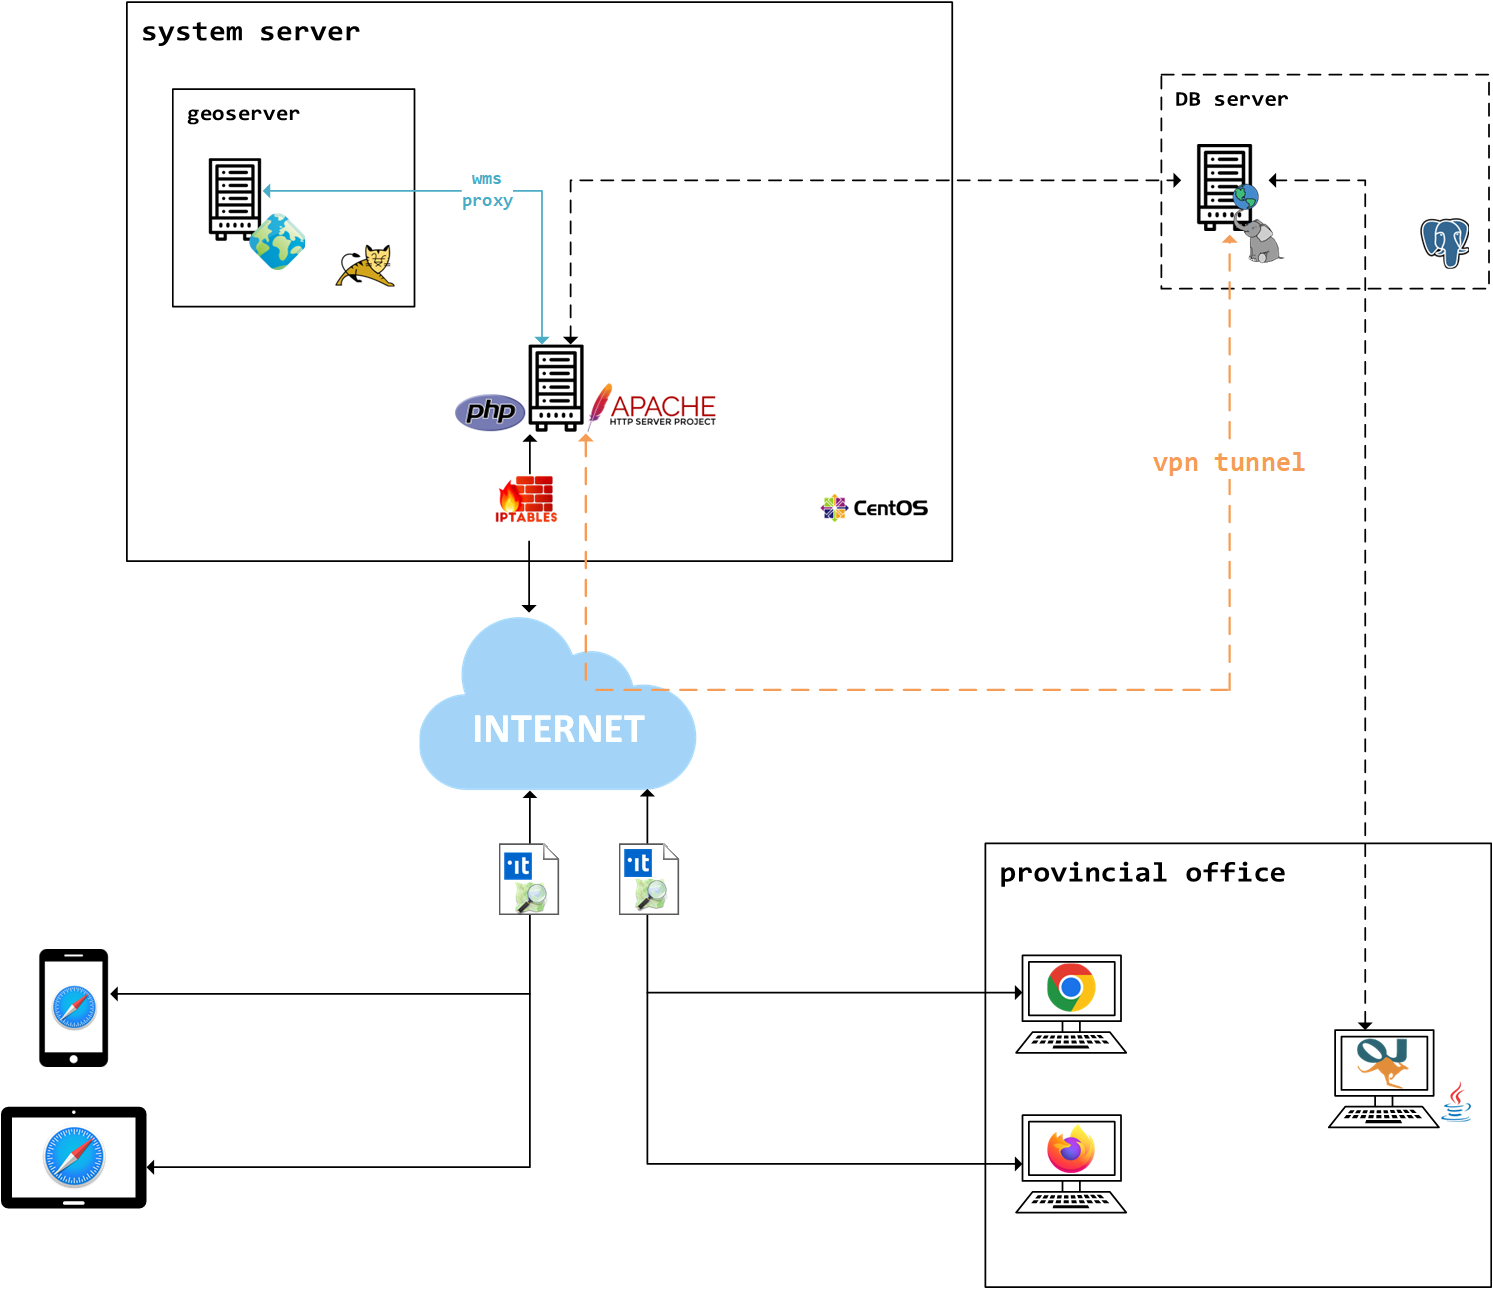
\includegraphics[width=\textwidth]{img/system}
    \caption{Logical schema}
    \label{LogicalSchema}
\end{figure}

\subsection{Functional Aspects of the System}
The systems are developed in a way that no specific capabilities are required from the users.
Anyway, here we provide some short explanation of some of the functionalities that we developed as a demo; the usability of the whole application will be based on the same technologies and possible to use in the same way. 
\subsubsection{WebGIS Application}
The web application shall be used both from the citizenship side (from mobile devices) and from the provincial technicians, that has to access to the web application from a desktop computer.
Starting from the perspective of the citizenship, the functionalities are:
\begin{itemize}
    \vspace{3ex}
    \item \textbf{Home page} \\
    \begin{figure}[H]\centering 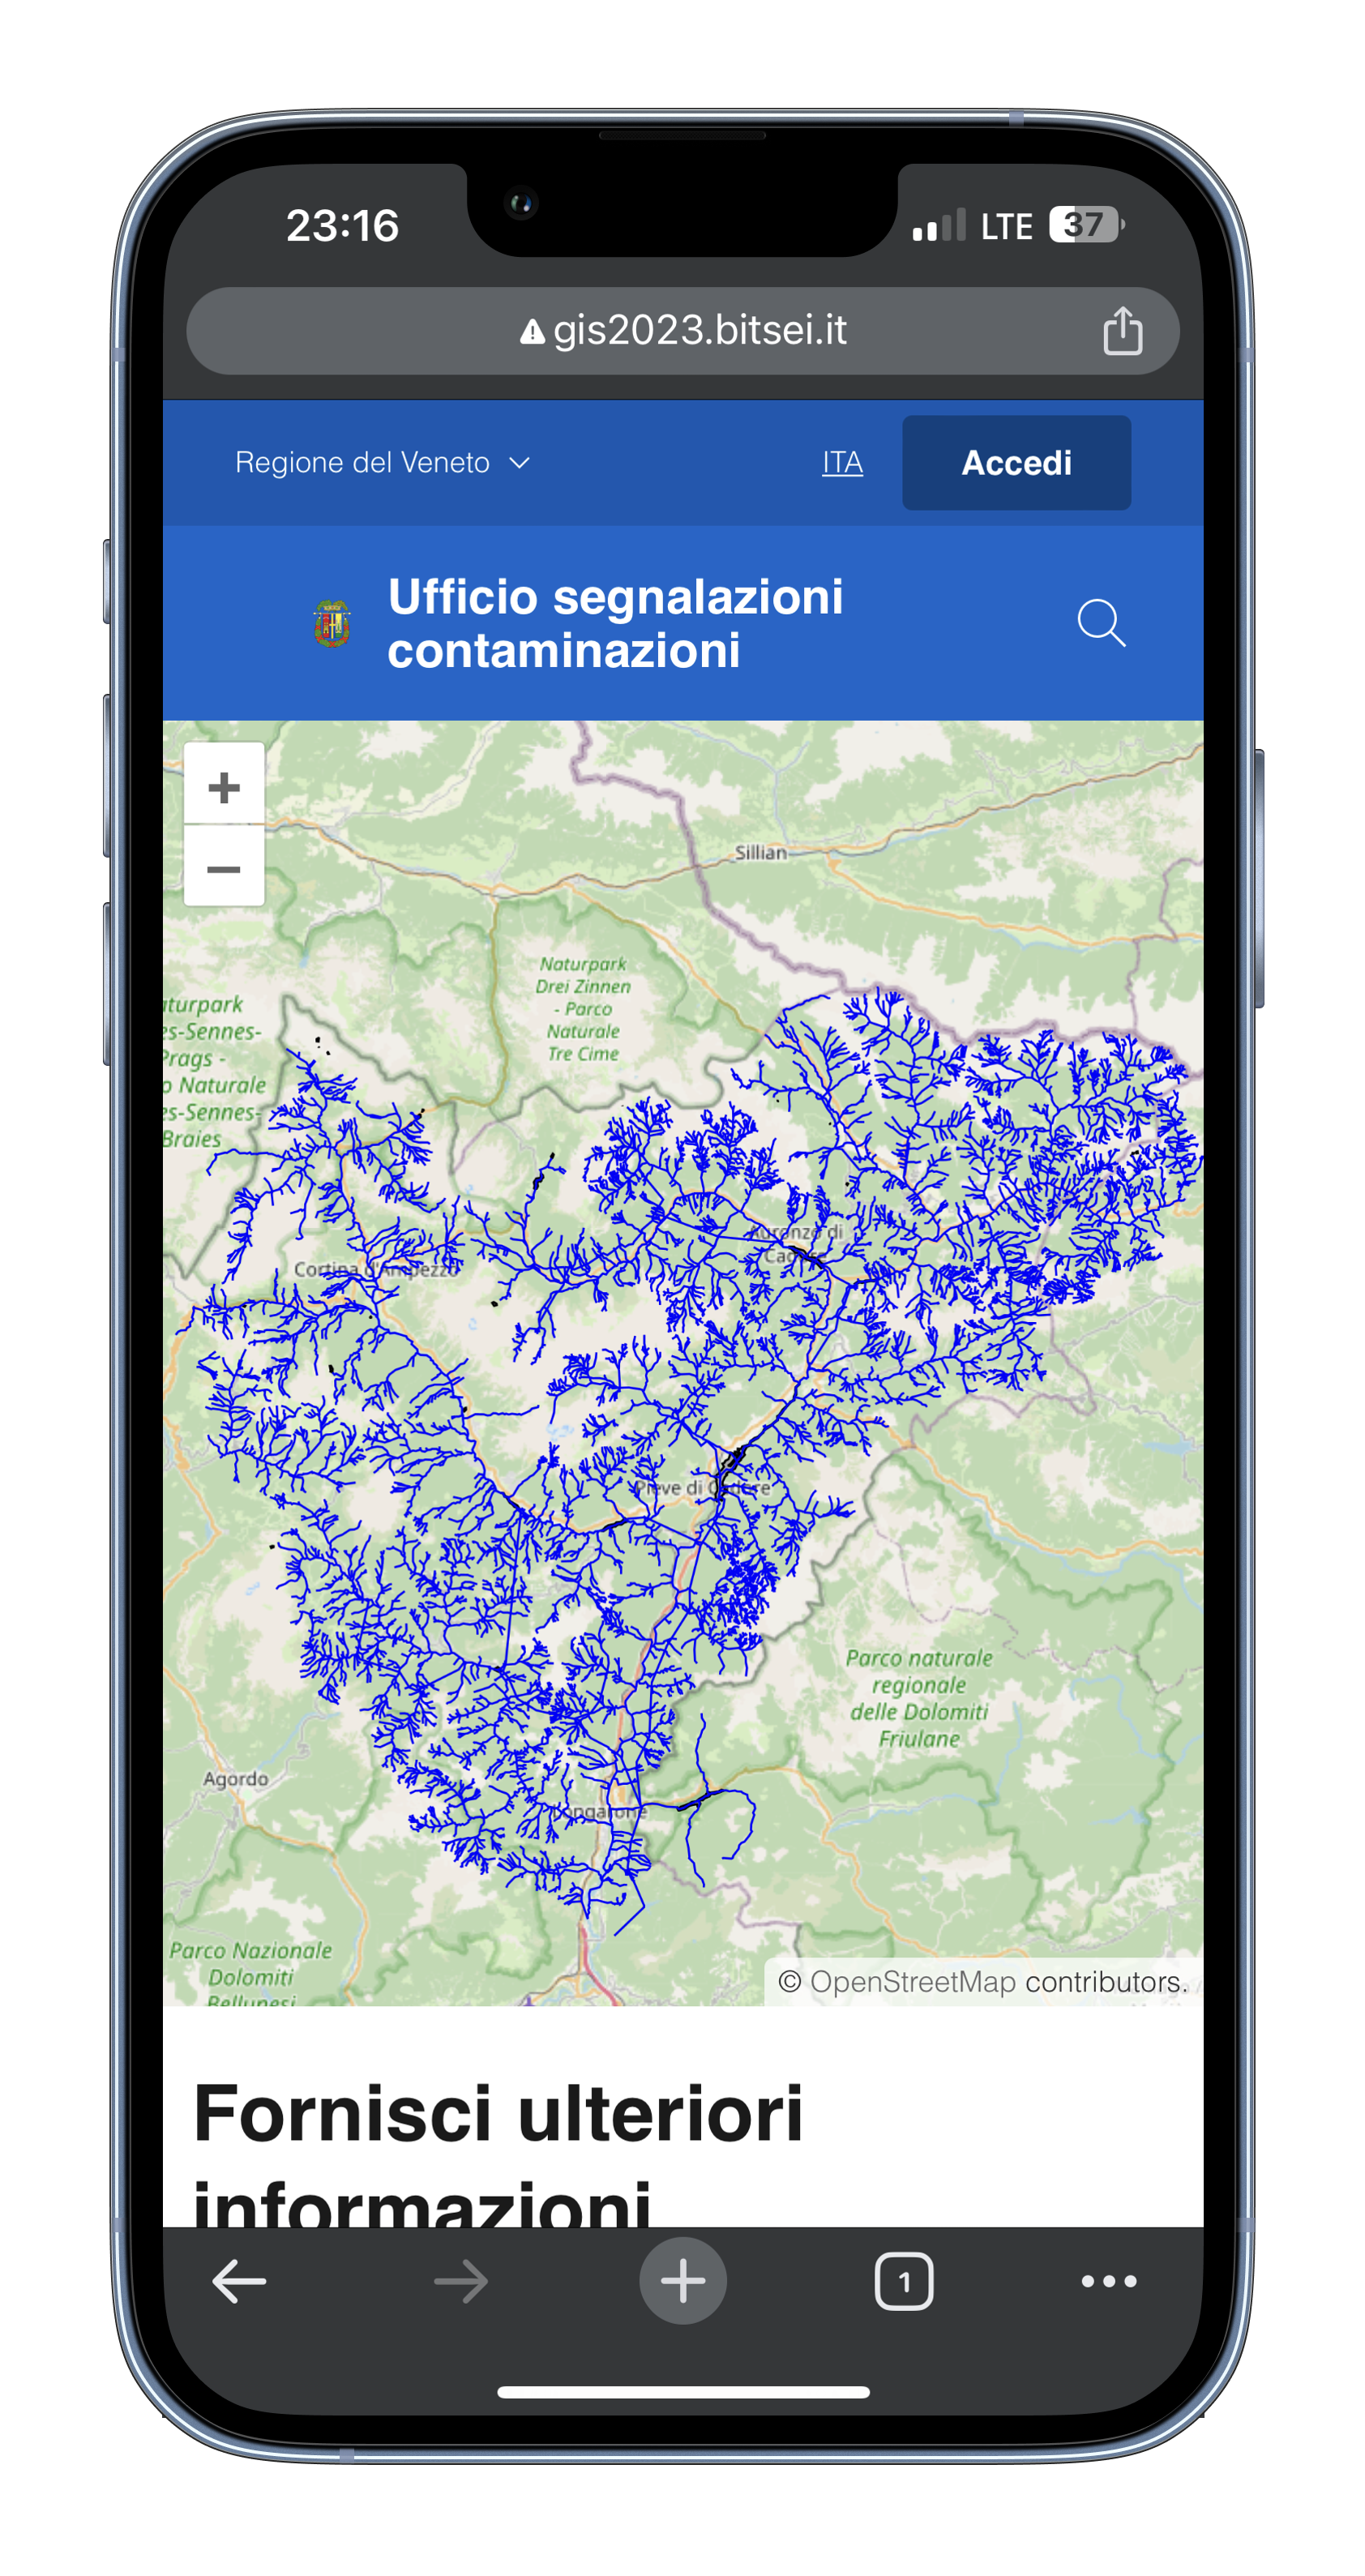
\includegraphics[width=12em]{img/home.png} 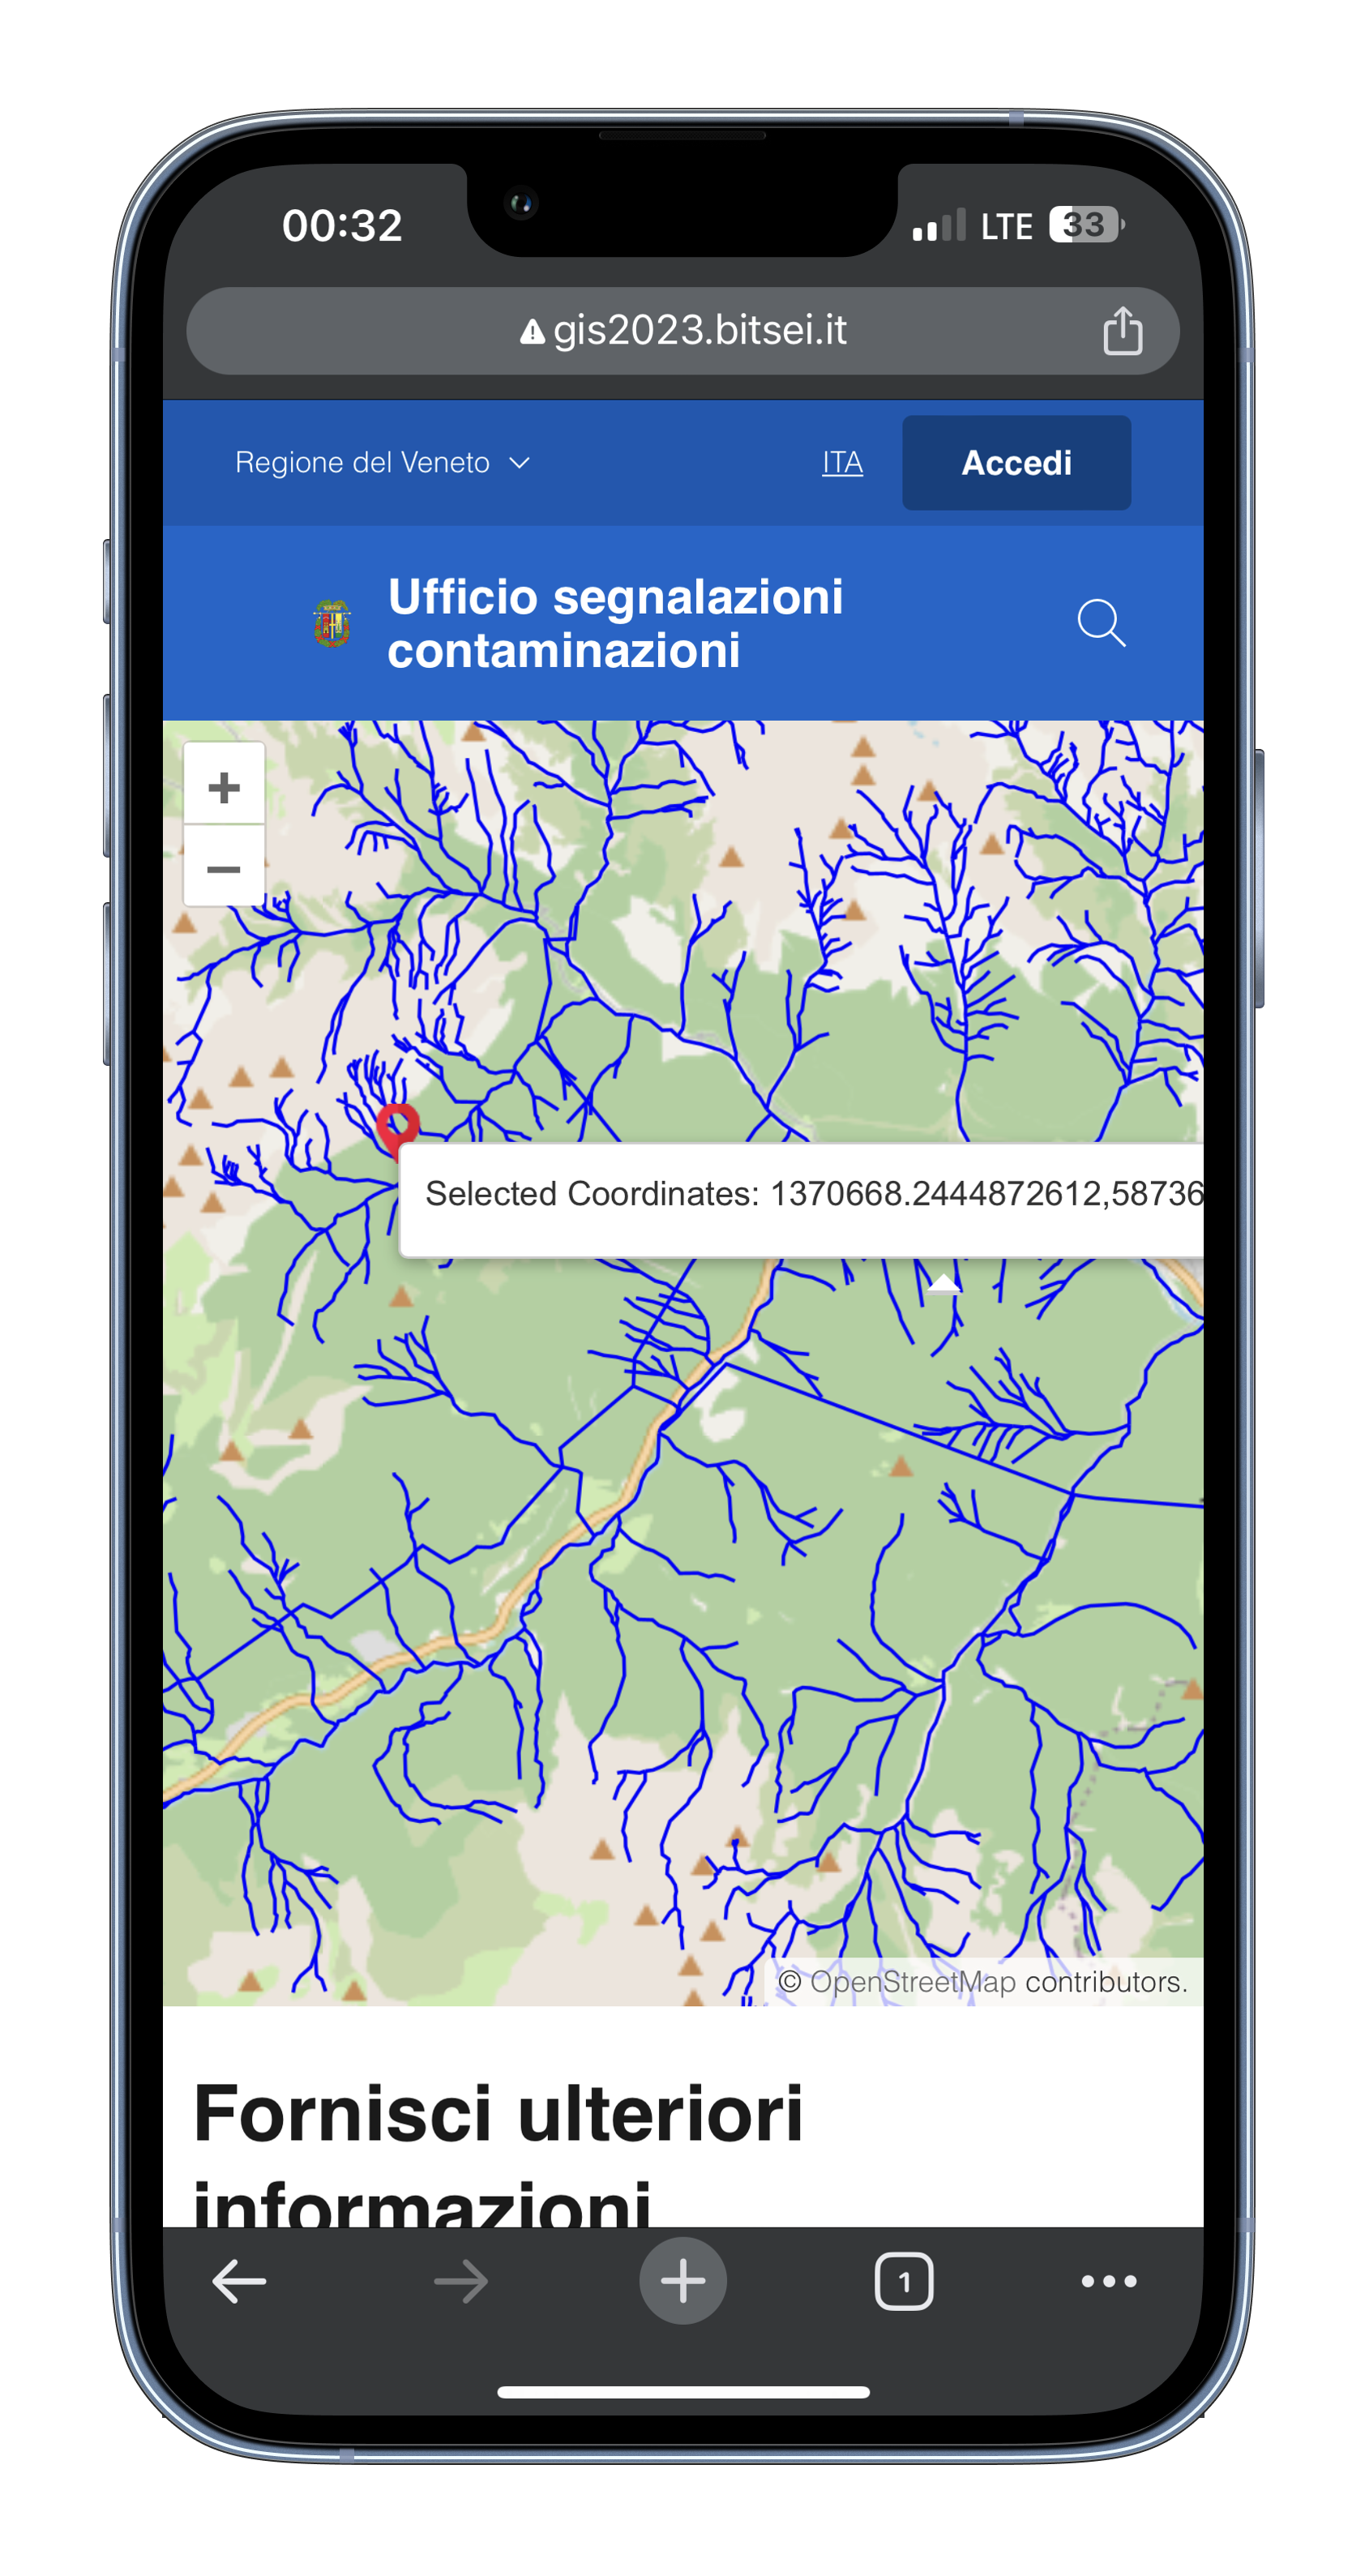
\includegraphics[width=12em]{img/posizione.png} 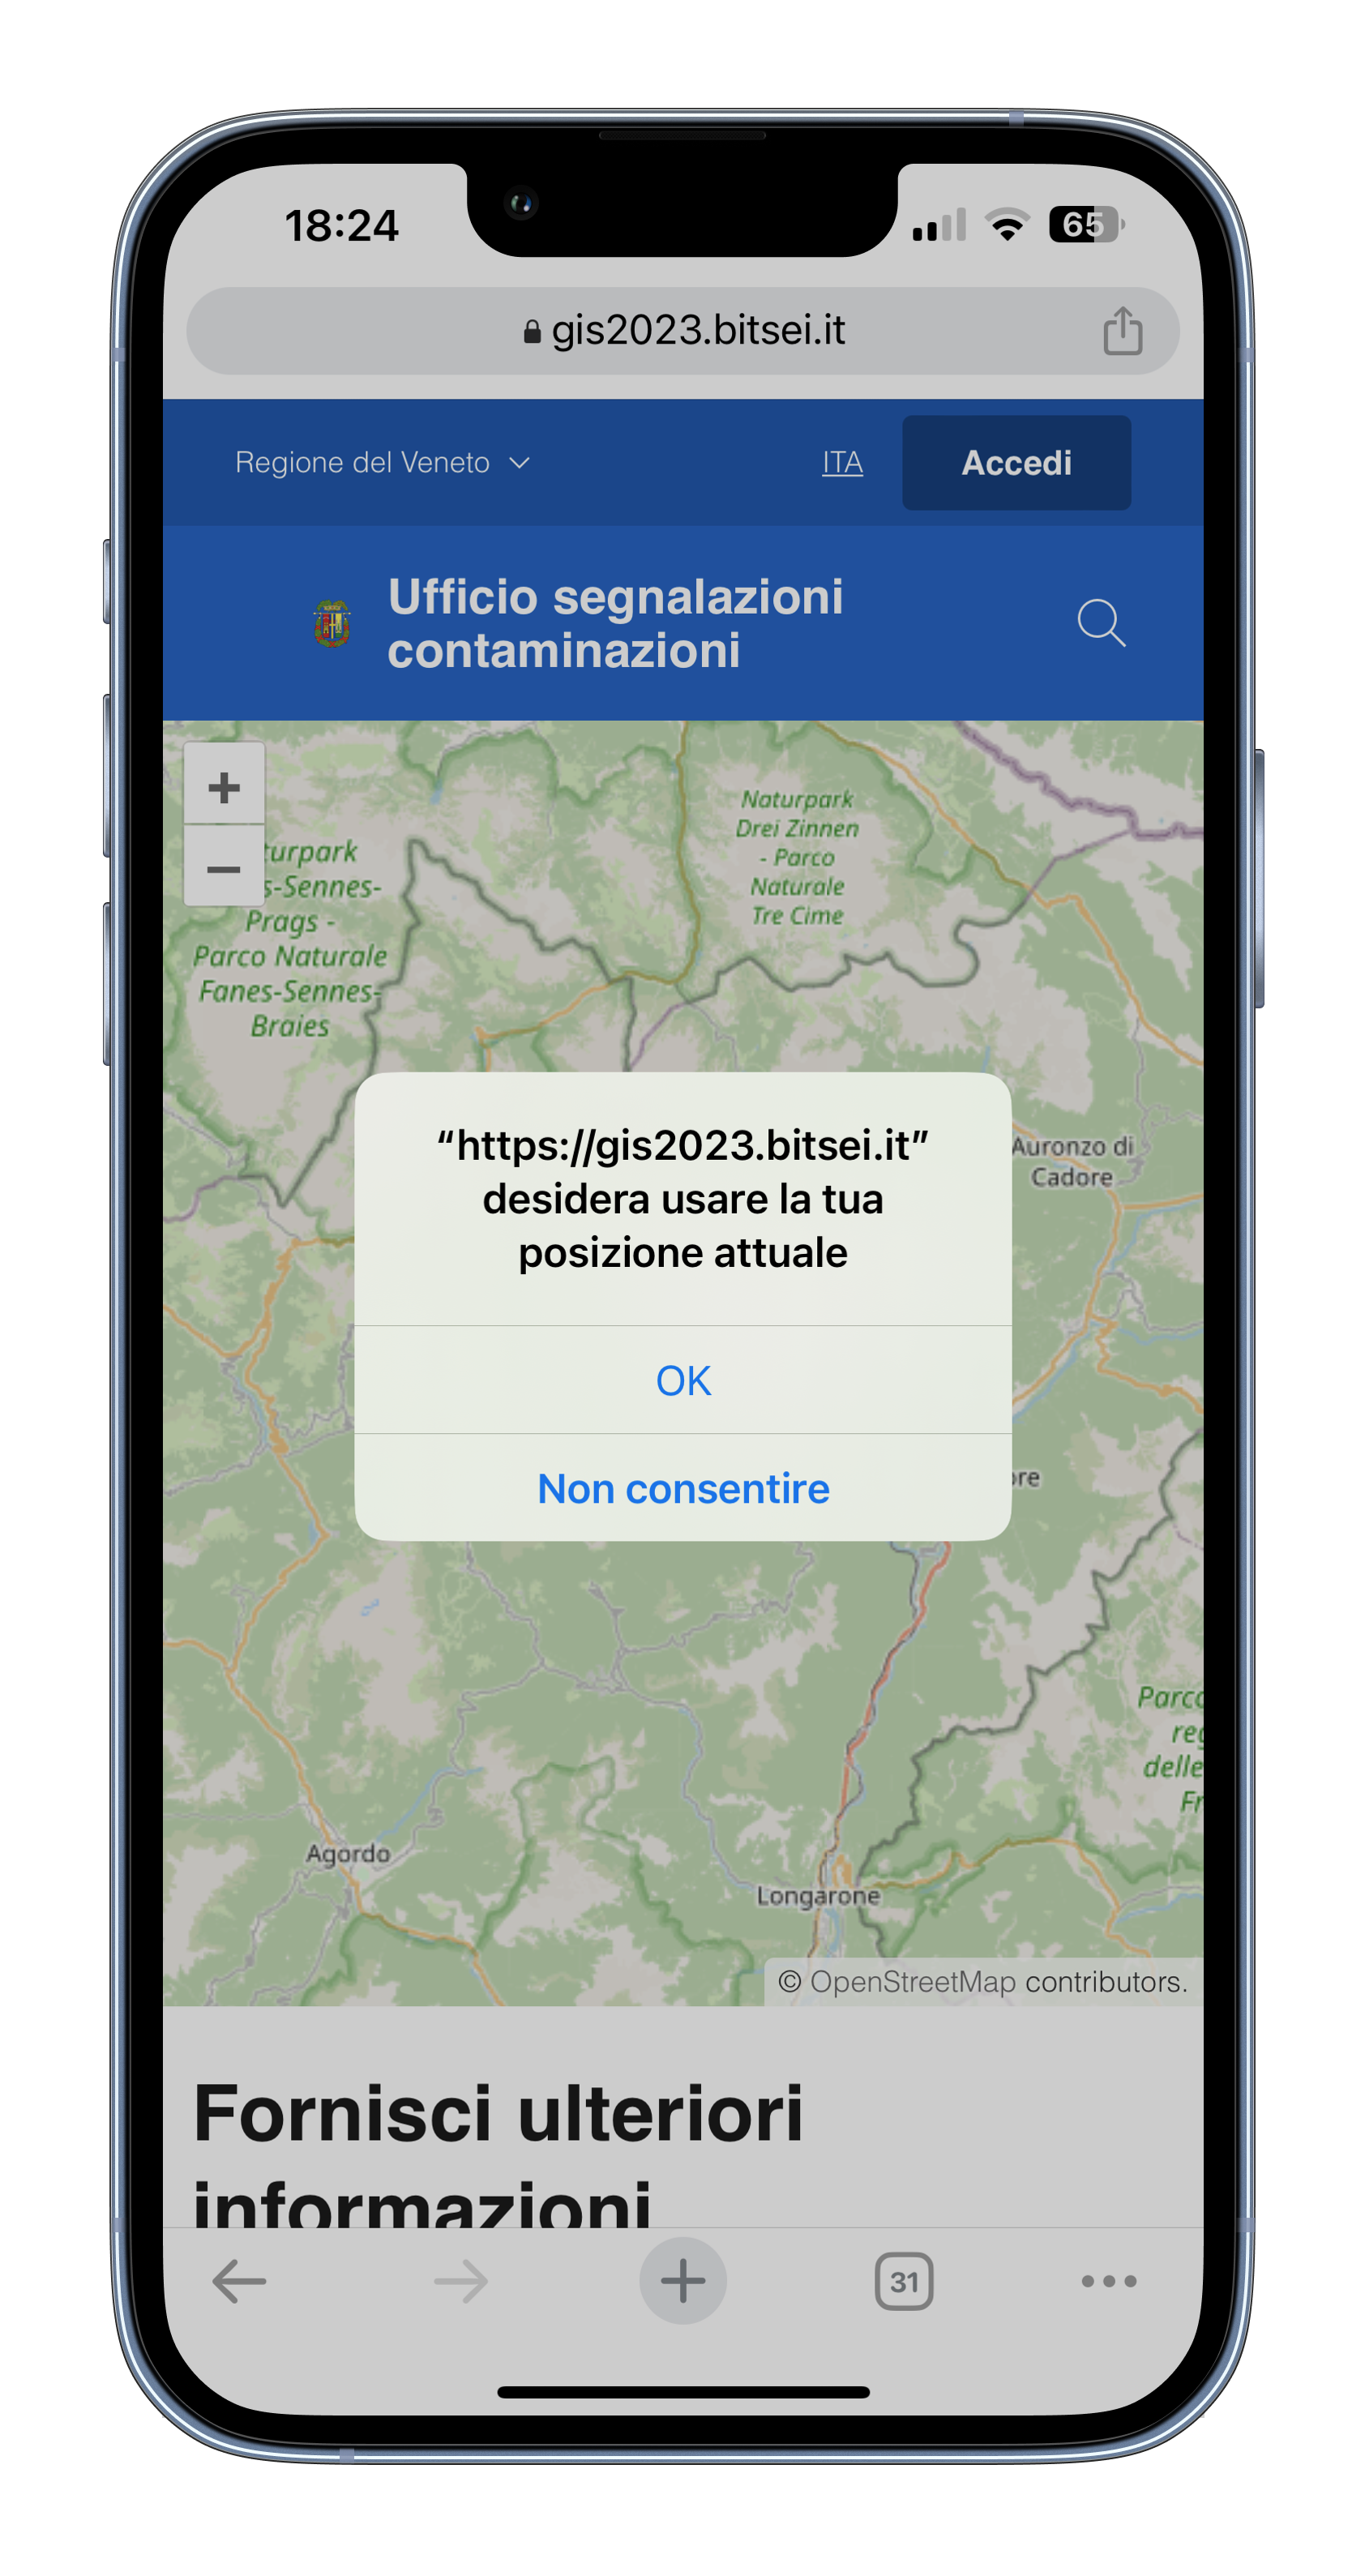
\includegraphics[width=12em]{img/autoposizione.png}  \caption{Smartphone map view} \label{phoneHomepage}\end{figure}
    The page loads showing as a background (under the headings) the map of the province of Belluno; the user can surf the map and select the position by clicking on it; when the page loads the first time, it asks the user to gather the position from the device, without the need of him to choose it manually Fig:[\ref{phoneHomepage}]. \\
    \pagebreak
    \item \textbf{Underlying form} \\
    \begin{figure}[H] \centering 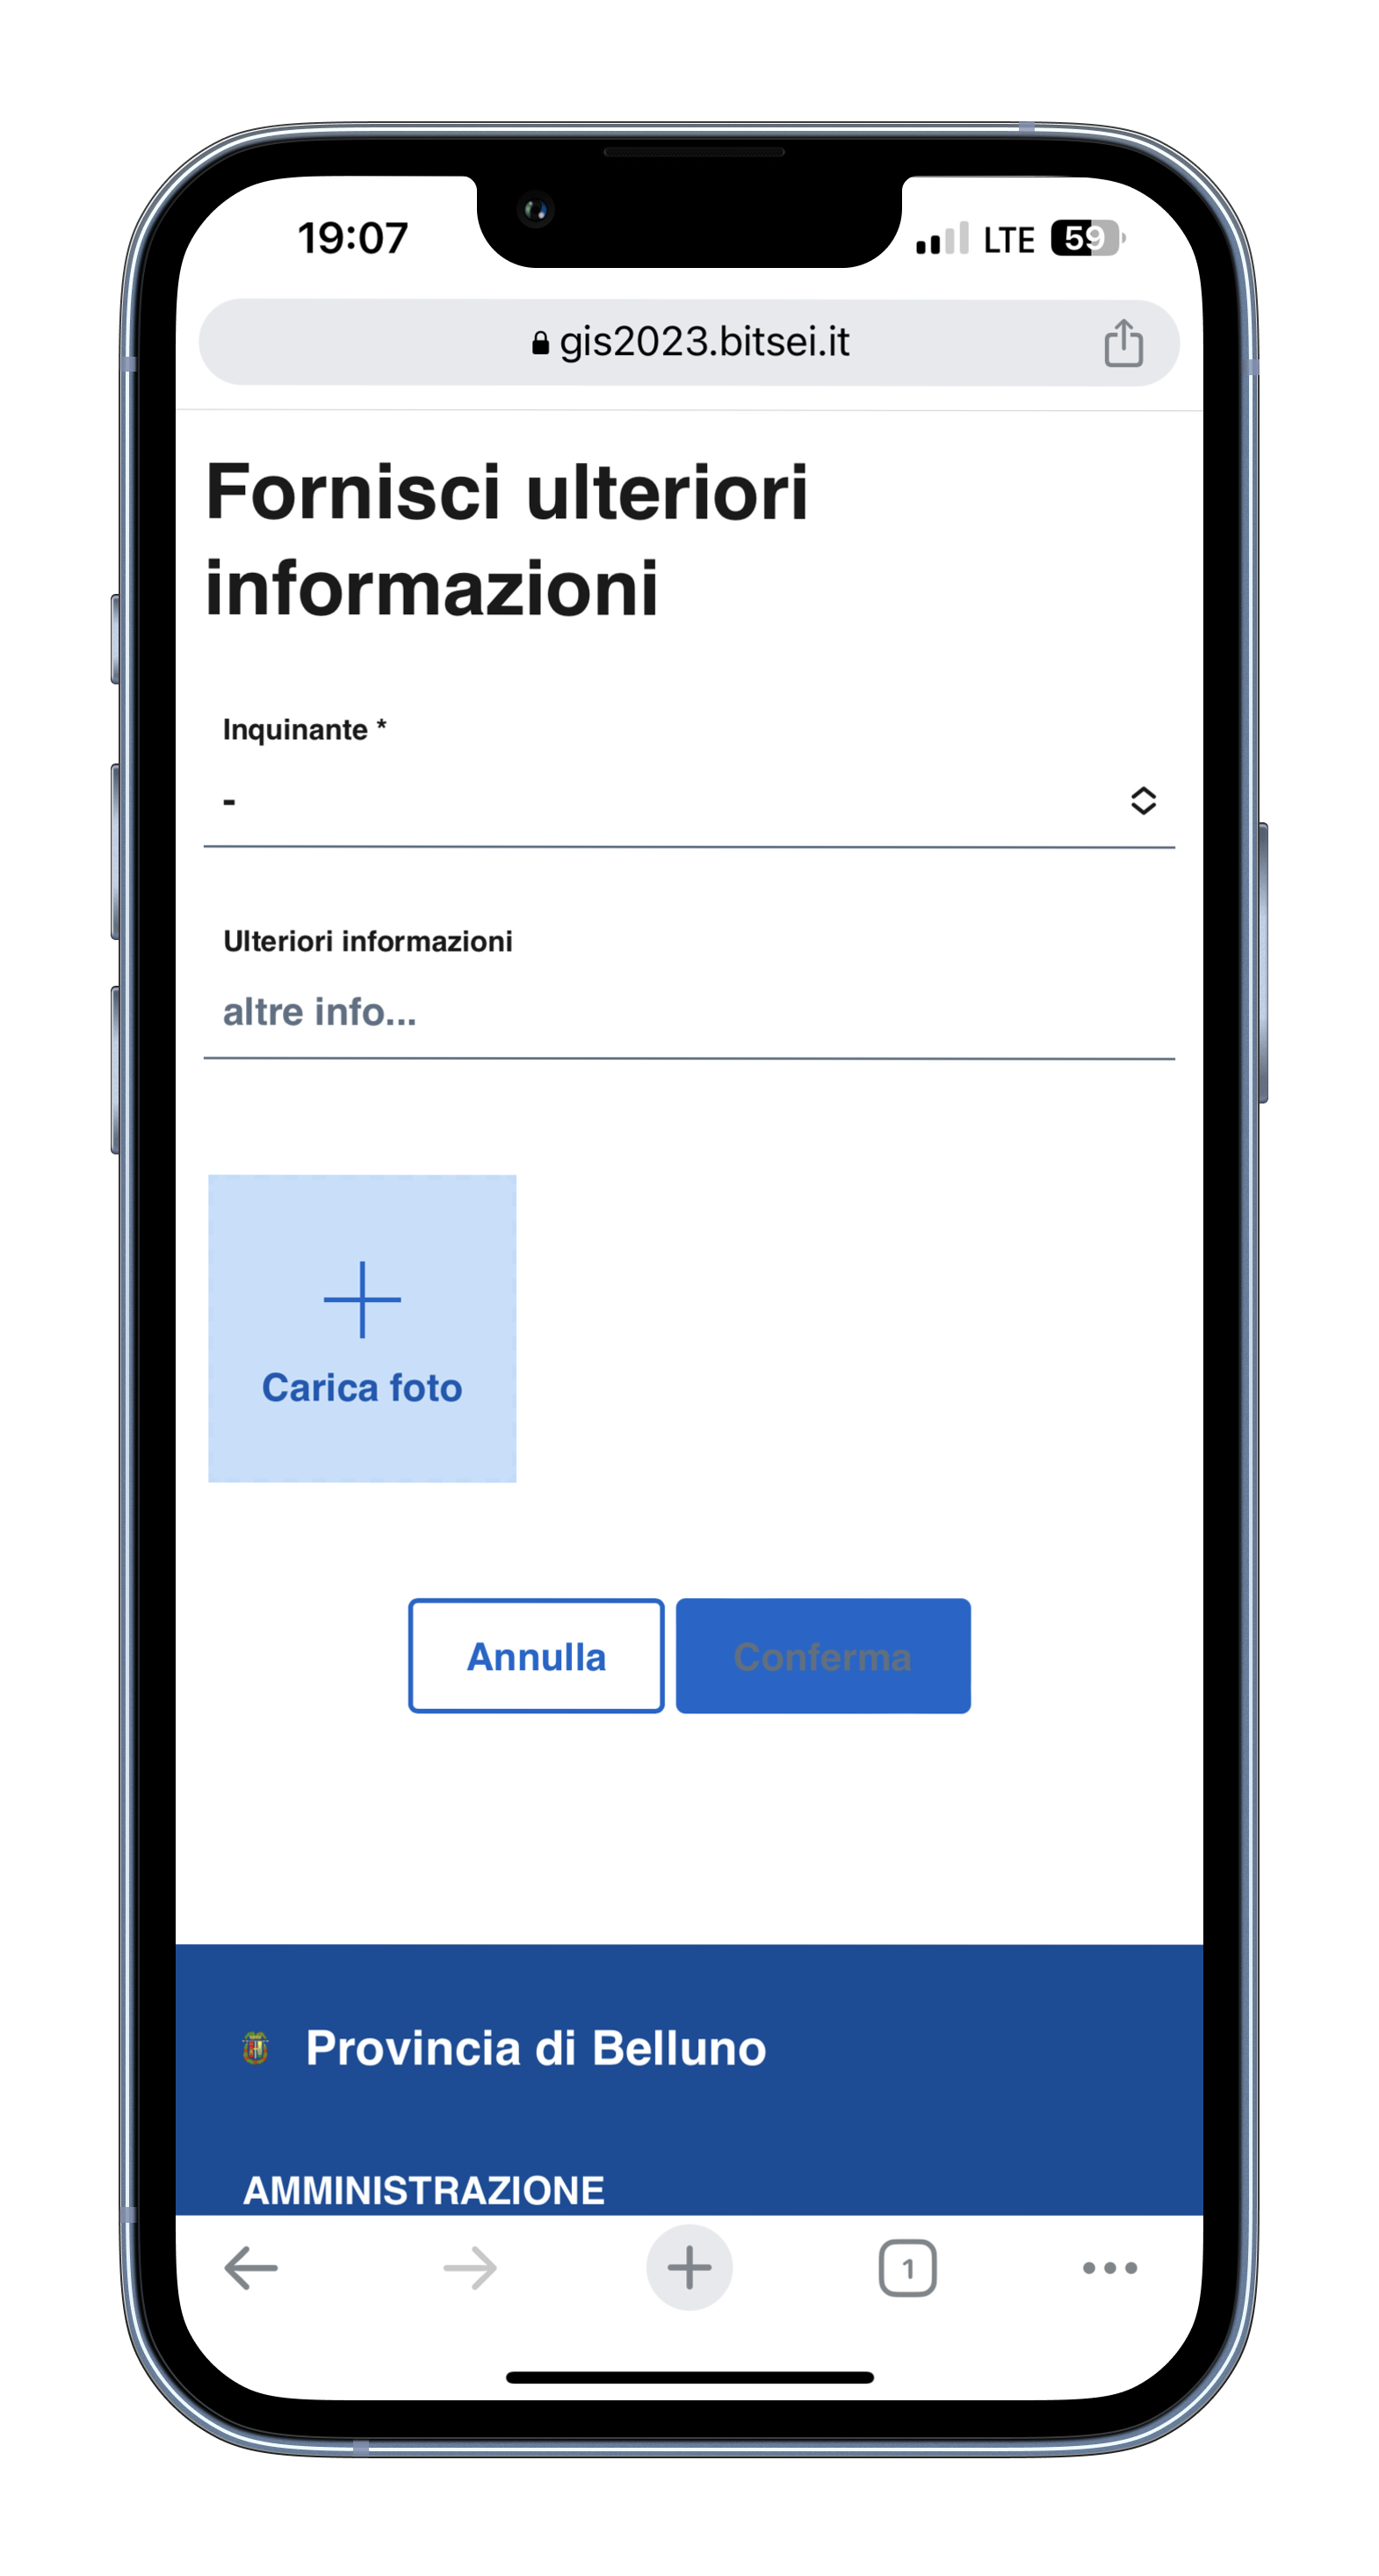
\includegraphics[width=12em]{img/form.png} 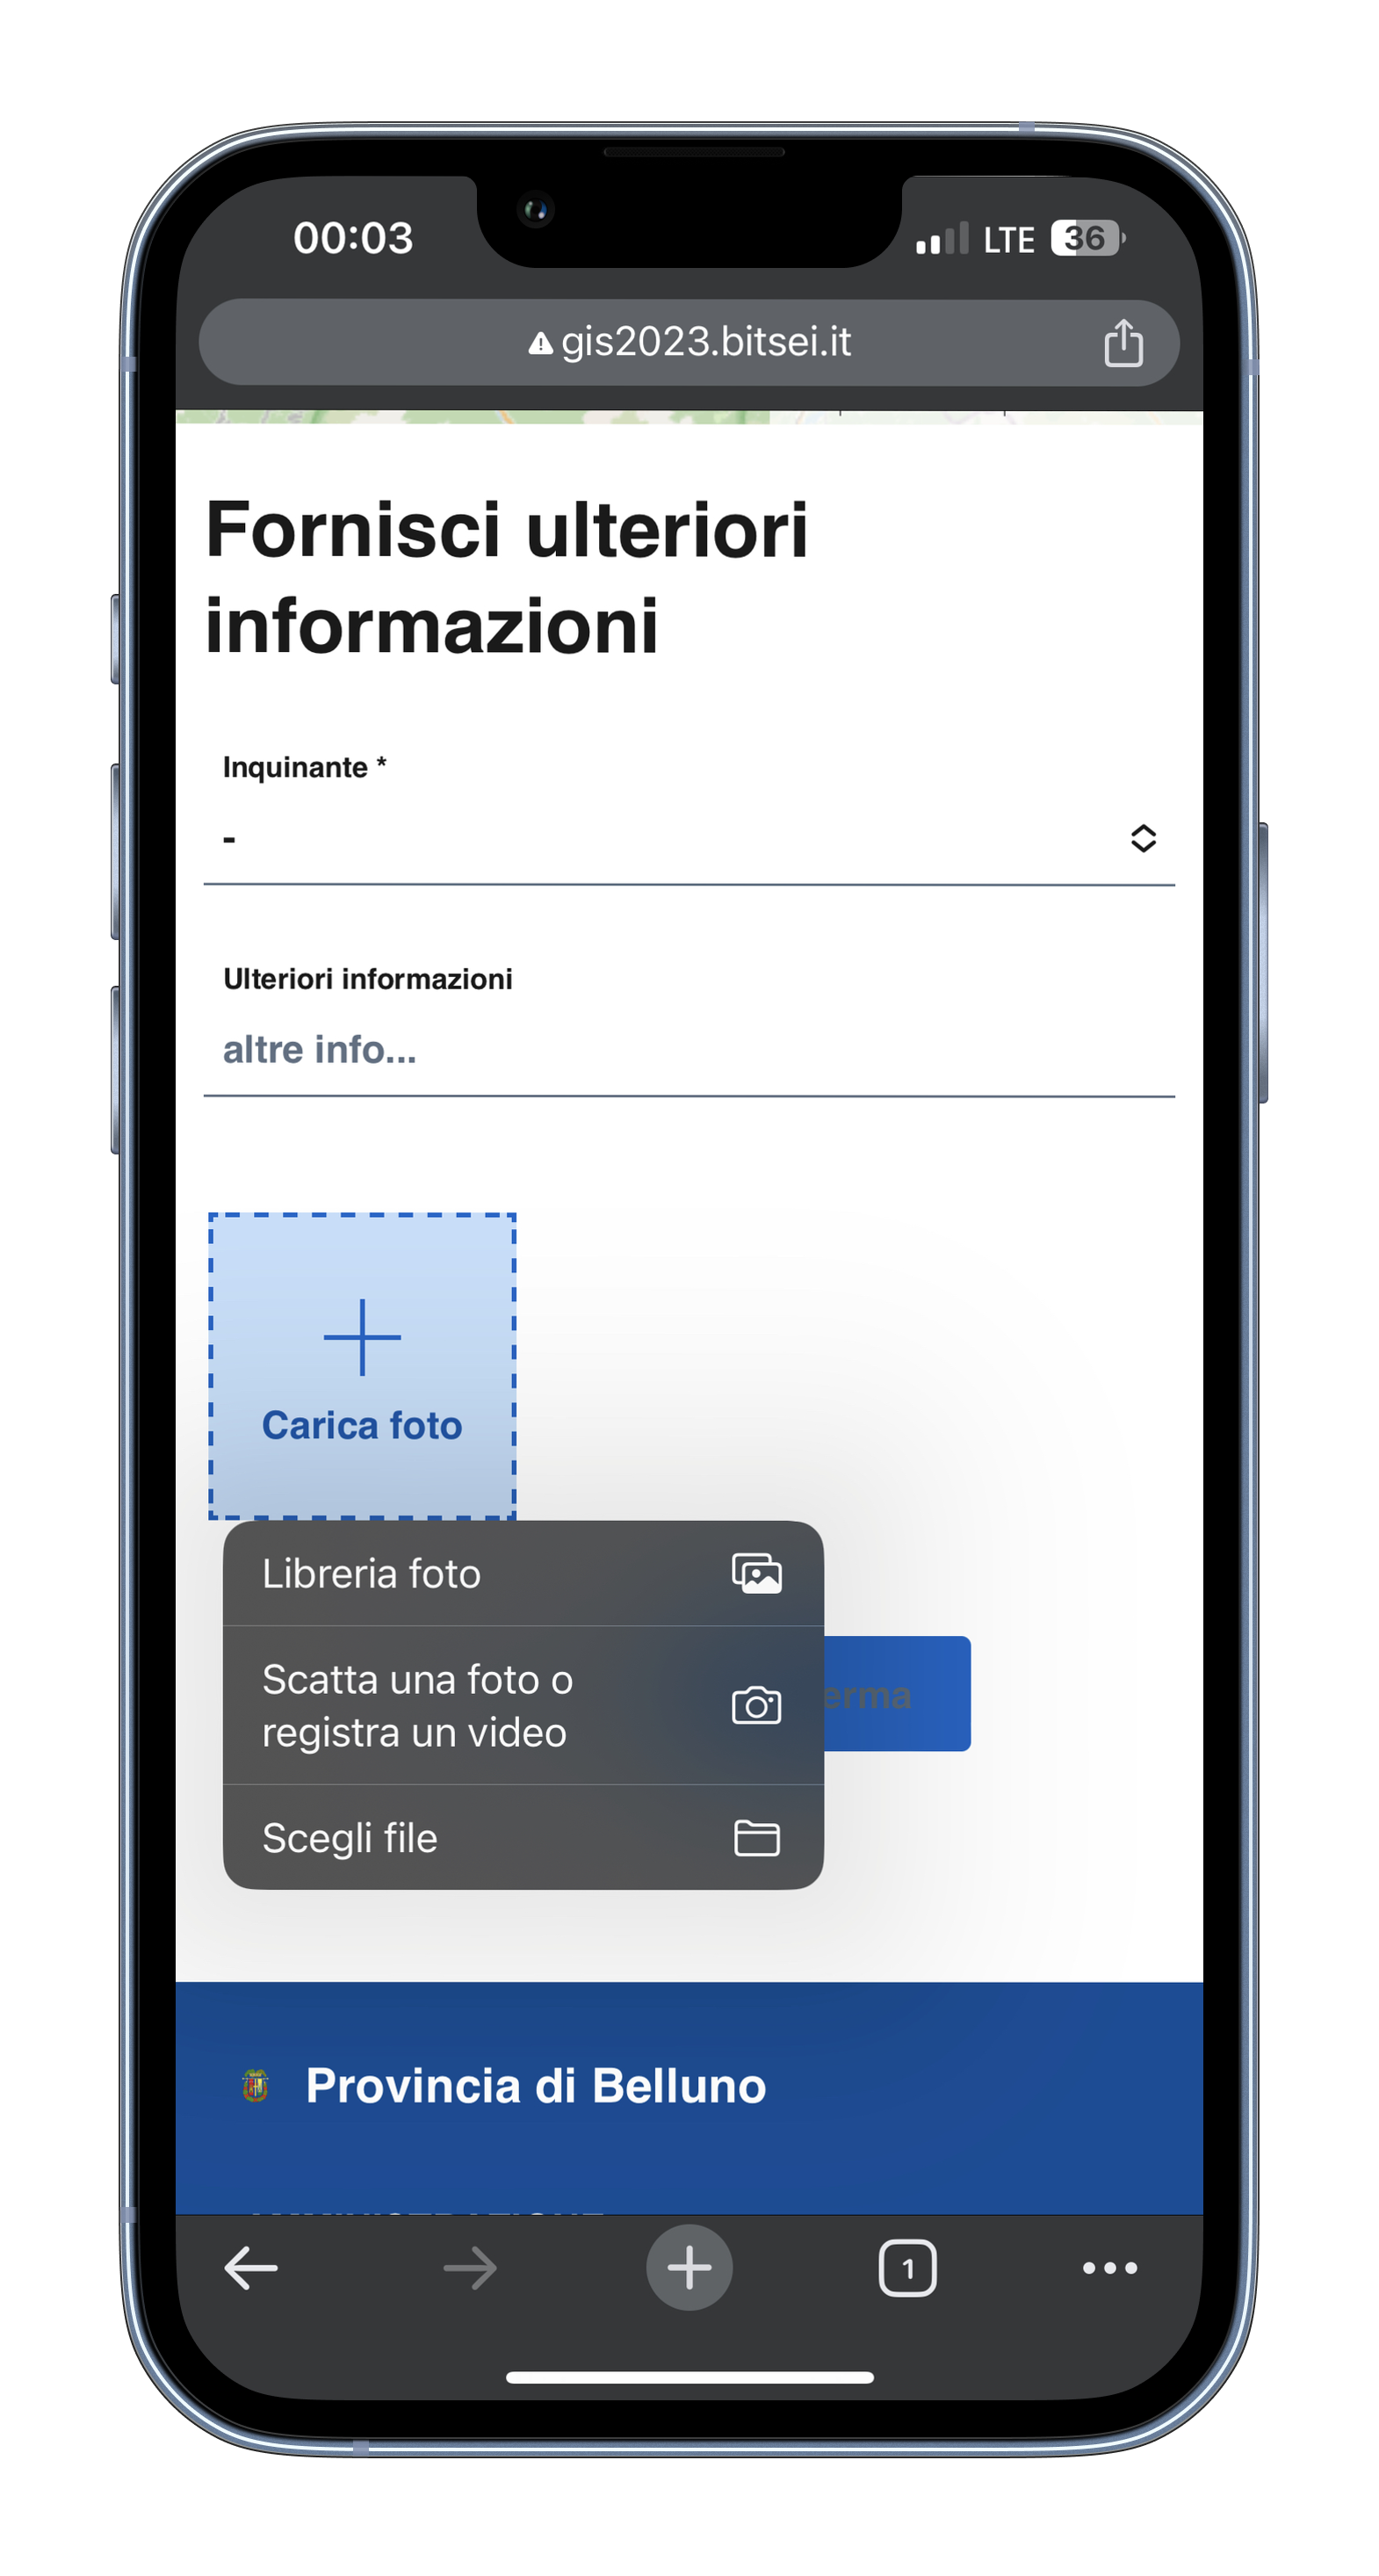
\includegraphics[width=12em]{img/foto.png} \caption{Smartphone view for uploading the the photo} \label{uploafPhoto} \end{figure}
    Under the map the user can fill the remaining form fields: he must select from a dropdown menu the pollutant found; he then can optionally write a description and upload an image, stored in its device or by capturing it from the camera [\ref{uploafPhoto}].
    \vspace{3ex}
    \item \textbf{Usability from a tablet} \\
    All the mentioned functionalities can be also used from a tablet rather than from a smartphones; the responsiveness is still guaranteed Fig[\ref{tablet}]: 
    \begin{figure}[H] \centering \includegraphics[width=24em]{img/tablet.png} \caption{Tablet interface} \label{tablet} \end{figure}
\end{itemize} 
\pagebreak
Switching to the perspective of the provincial technicians we have the following pages and functionalities:
\begin{itemize}
    \item \textbf{Login page} \\
    \begin{figure}[H]\centering 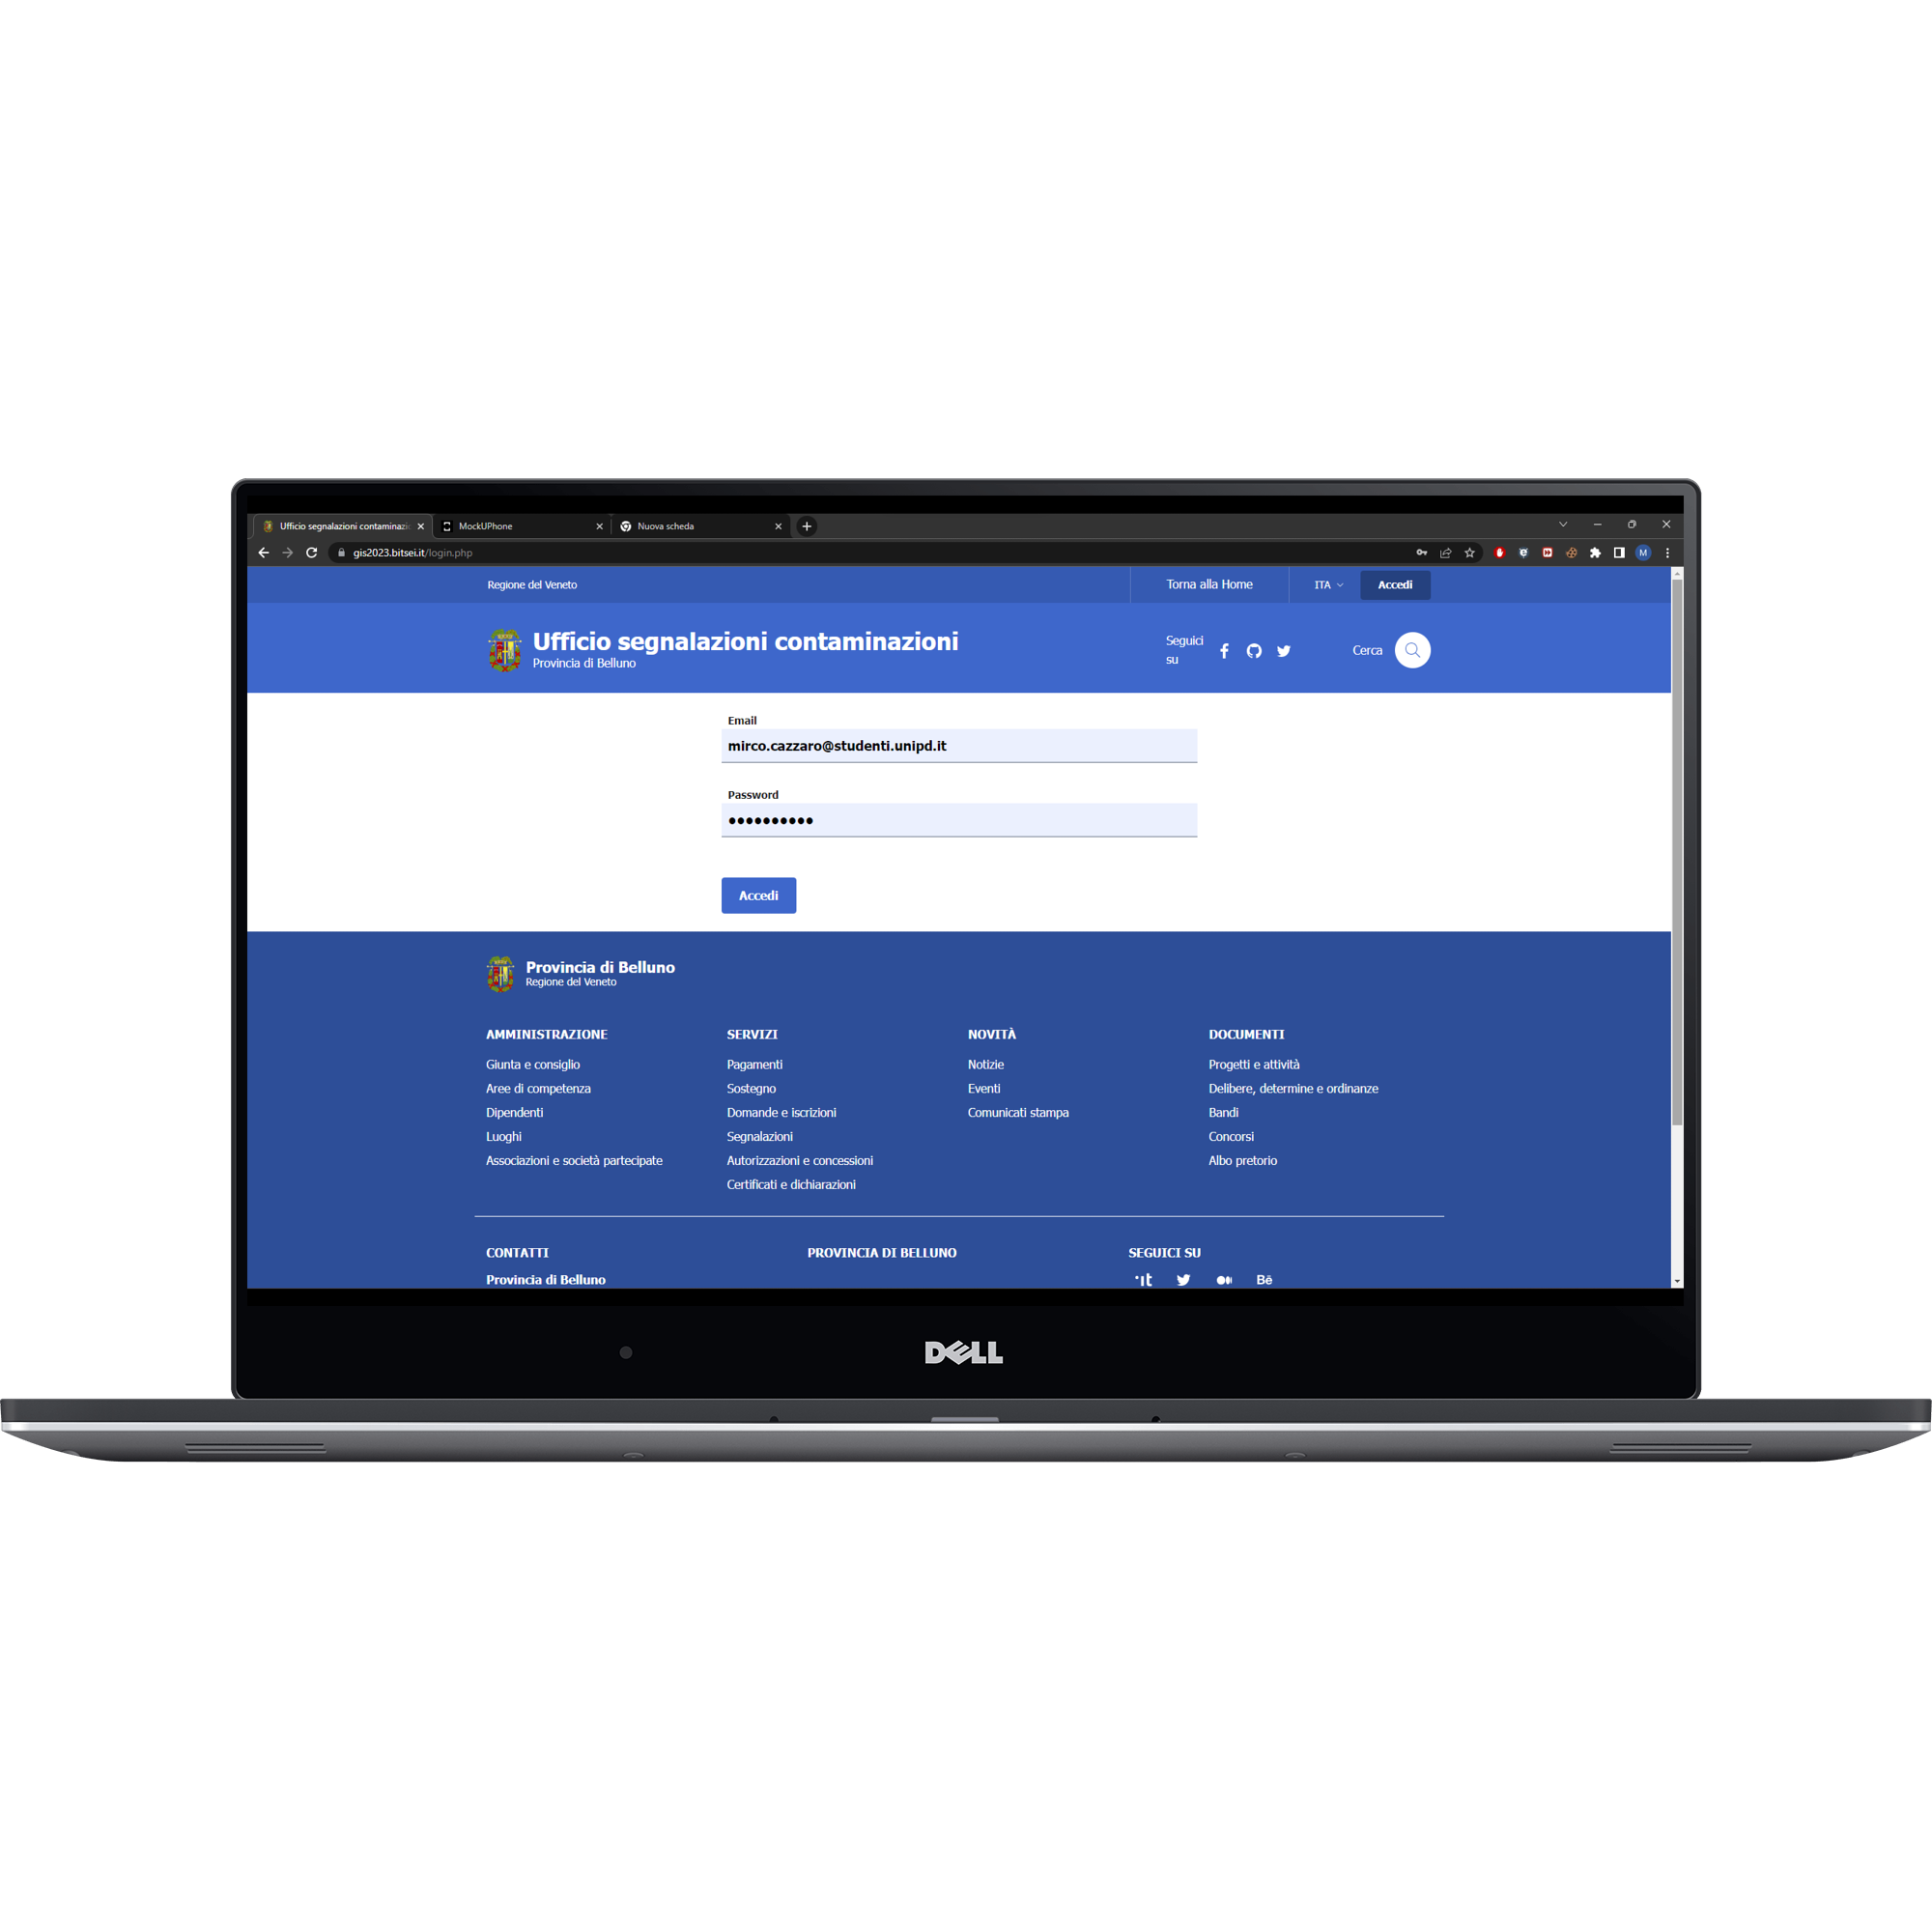
\includegraphics[width=27em]{img/login.png} \caption{Login page} \label{login} \end{figure}
    By pressing the button \textit{Accedi} on the top bar Fig[\ref{login}], we can access to the backend area reserved for the provincial technicians.
    If the login is successful a session is instantiated for the user, and he is redirected to a page that lists all the reports inserted by the citizens, filtered by year [\ref{backendListing}].
    \begin{figure}[H] \centering 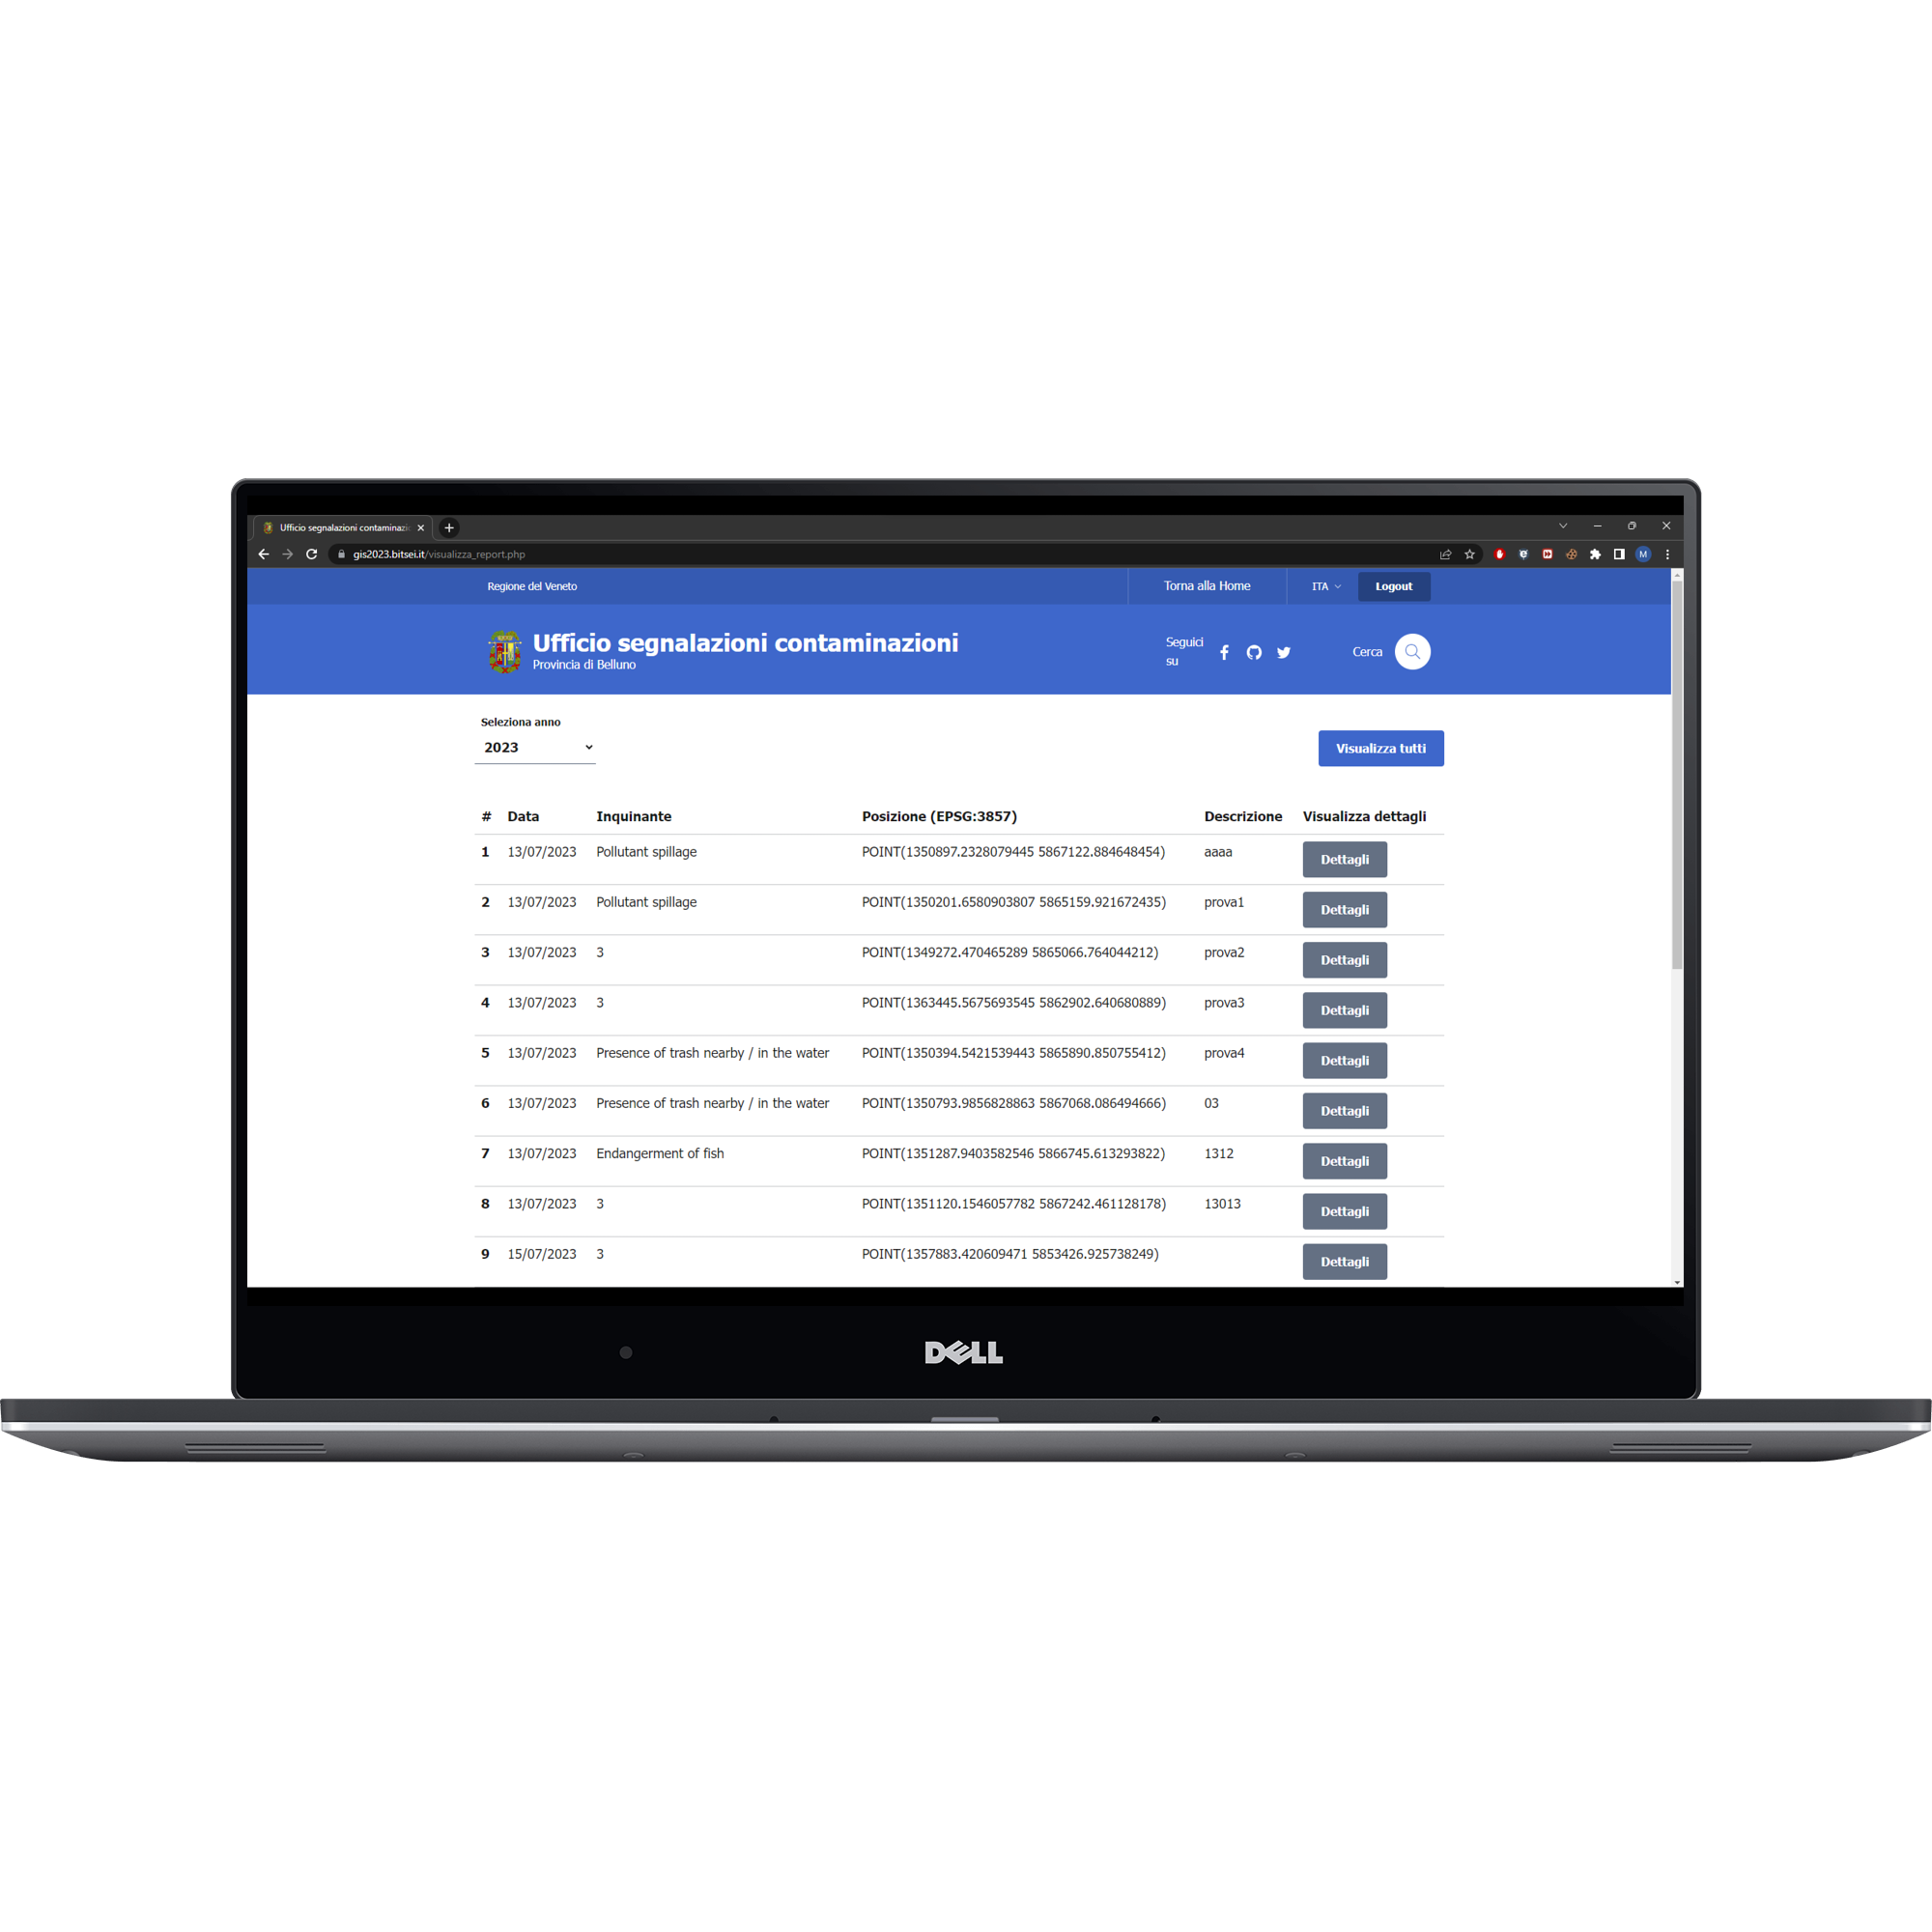
\includegraphics[width=27em]{img/home_back.png} \caption{Backend report listing} \label{backendListing}\end{figure}
    From here, an endpoint (button \textit{Dettagli}) showing a series of details is available for each report Fig[\ref{reportView}]:
    \begin{enumerate}
        \item the position;
        \item the pollutant selected;
        \item the date of the report;
        \item the optional description;
        \item the optional photo;
        \item the elevation from the level of the sea of the position.
    \end{enumerate}
    \begin{figure}[H] \centering 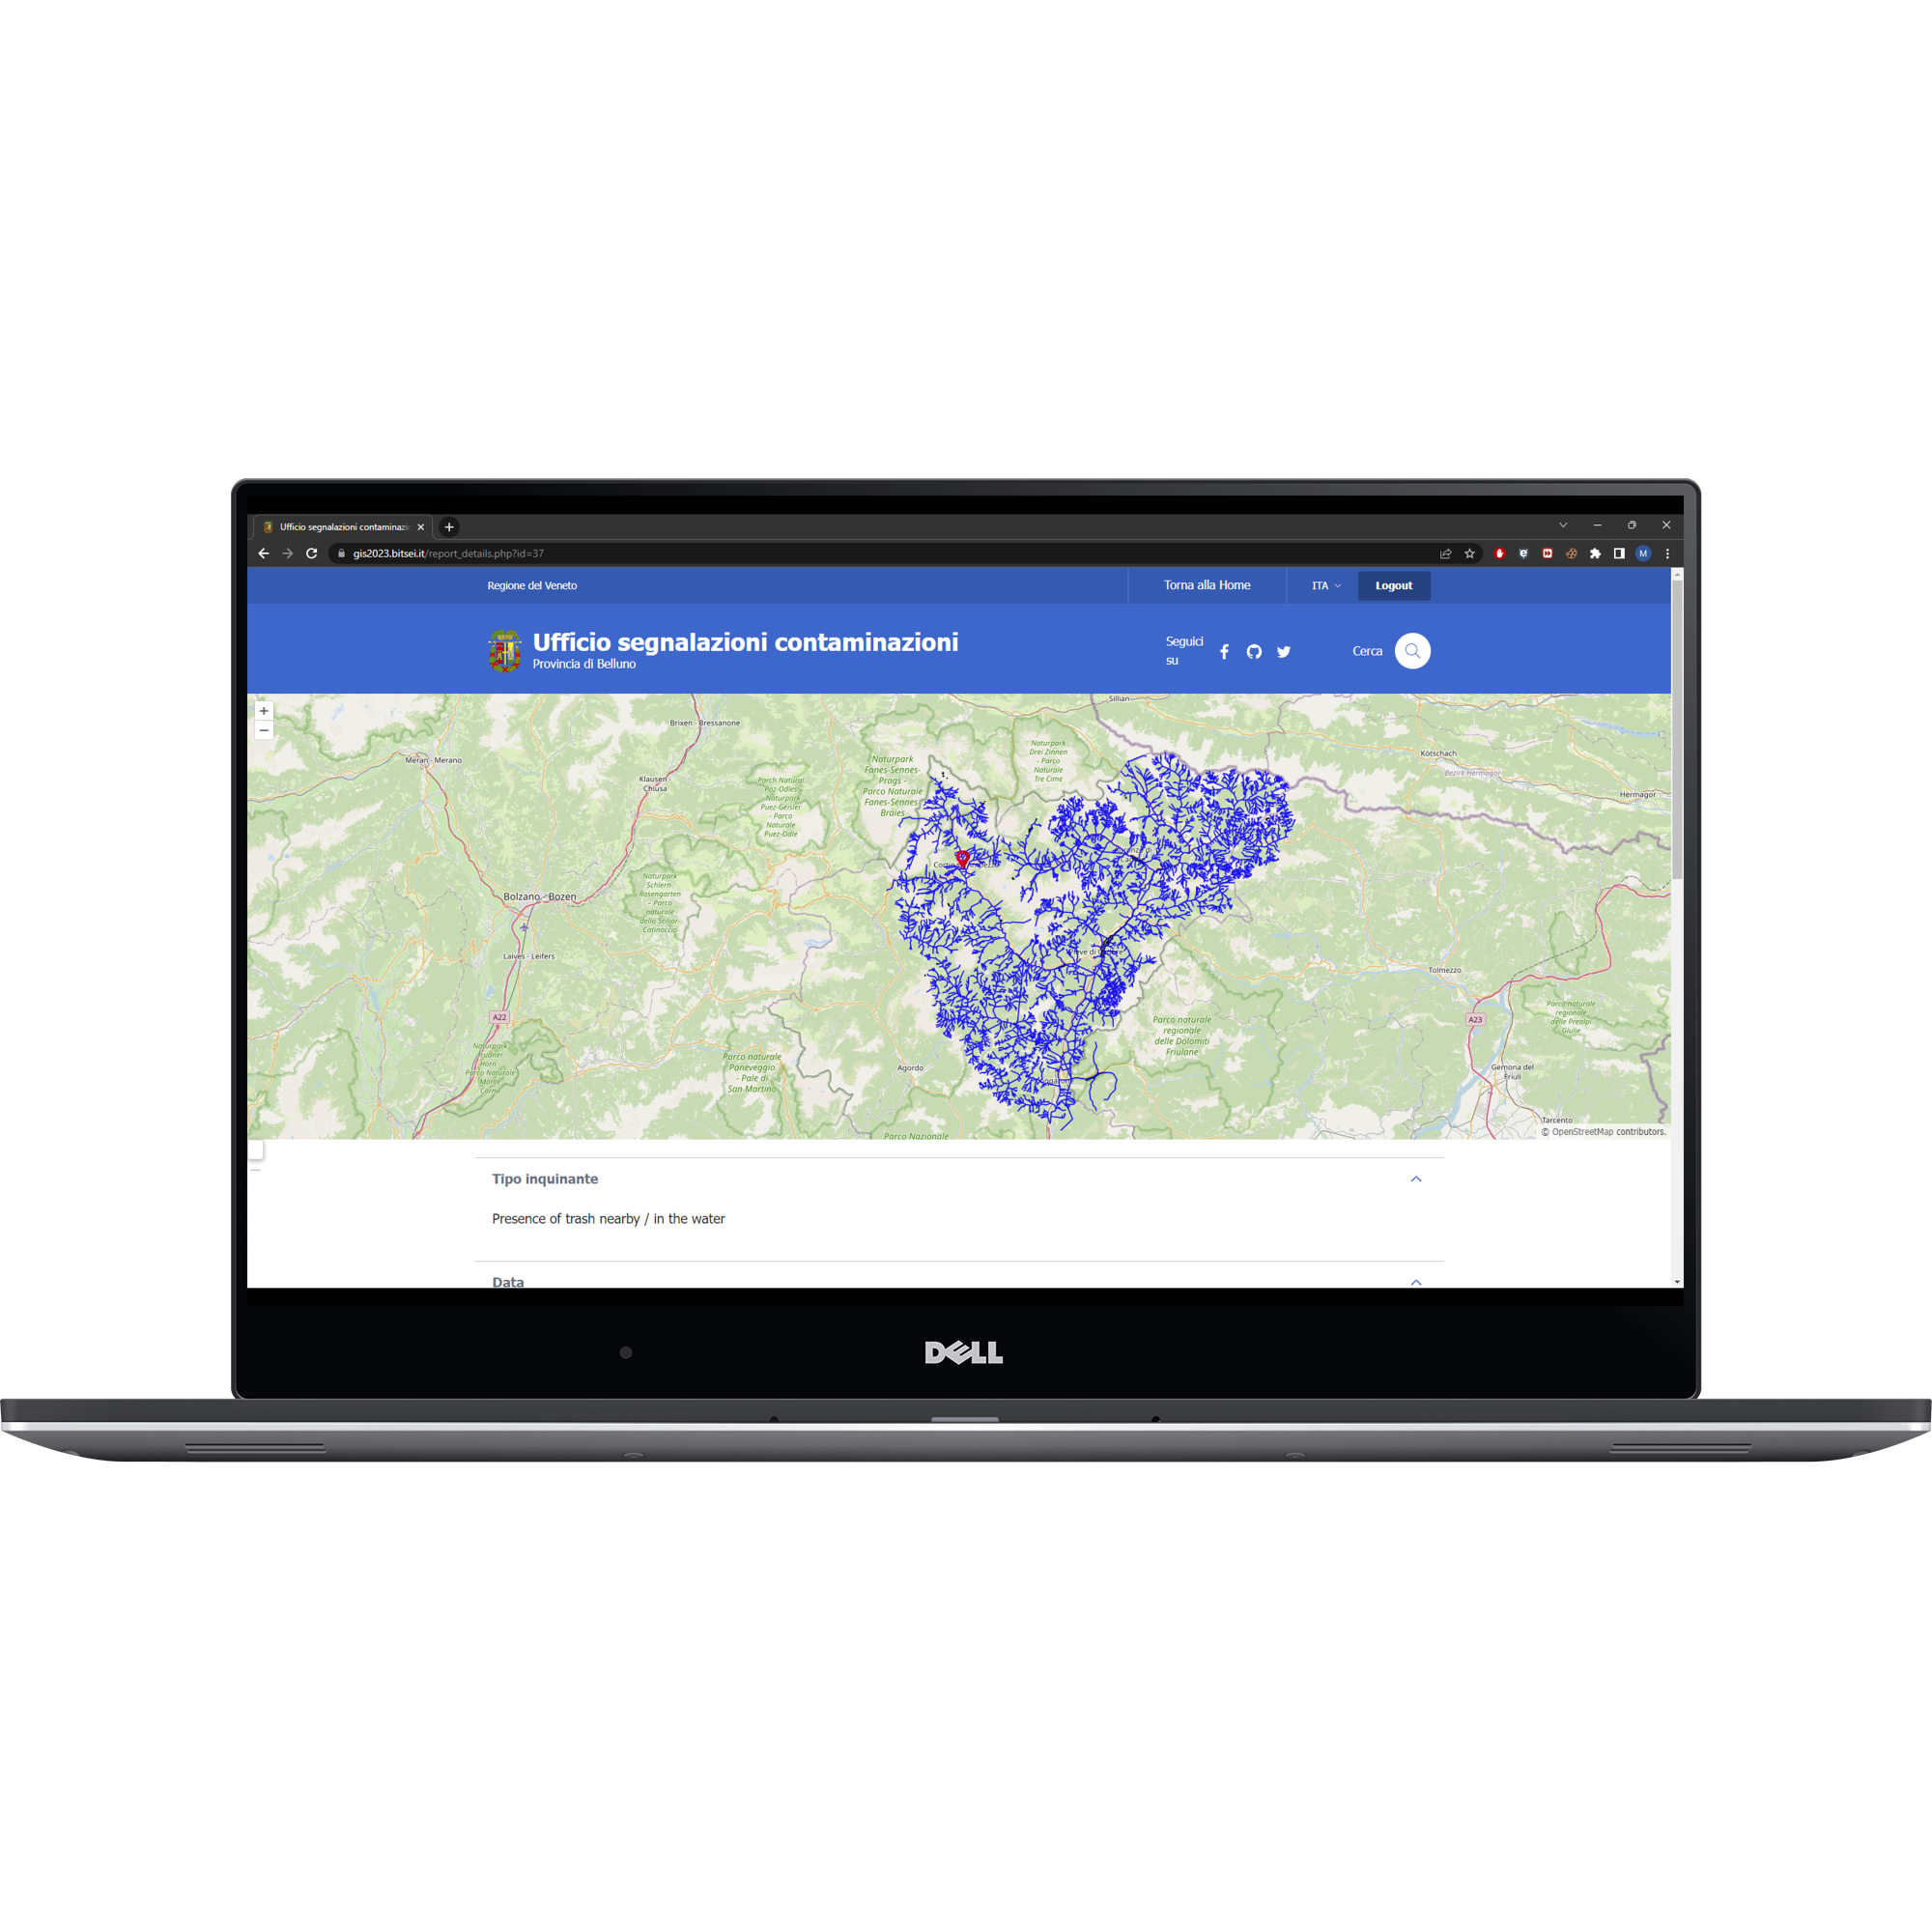
\includegraphics[width=27em]{img/pos_rep.png} 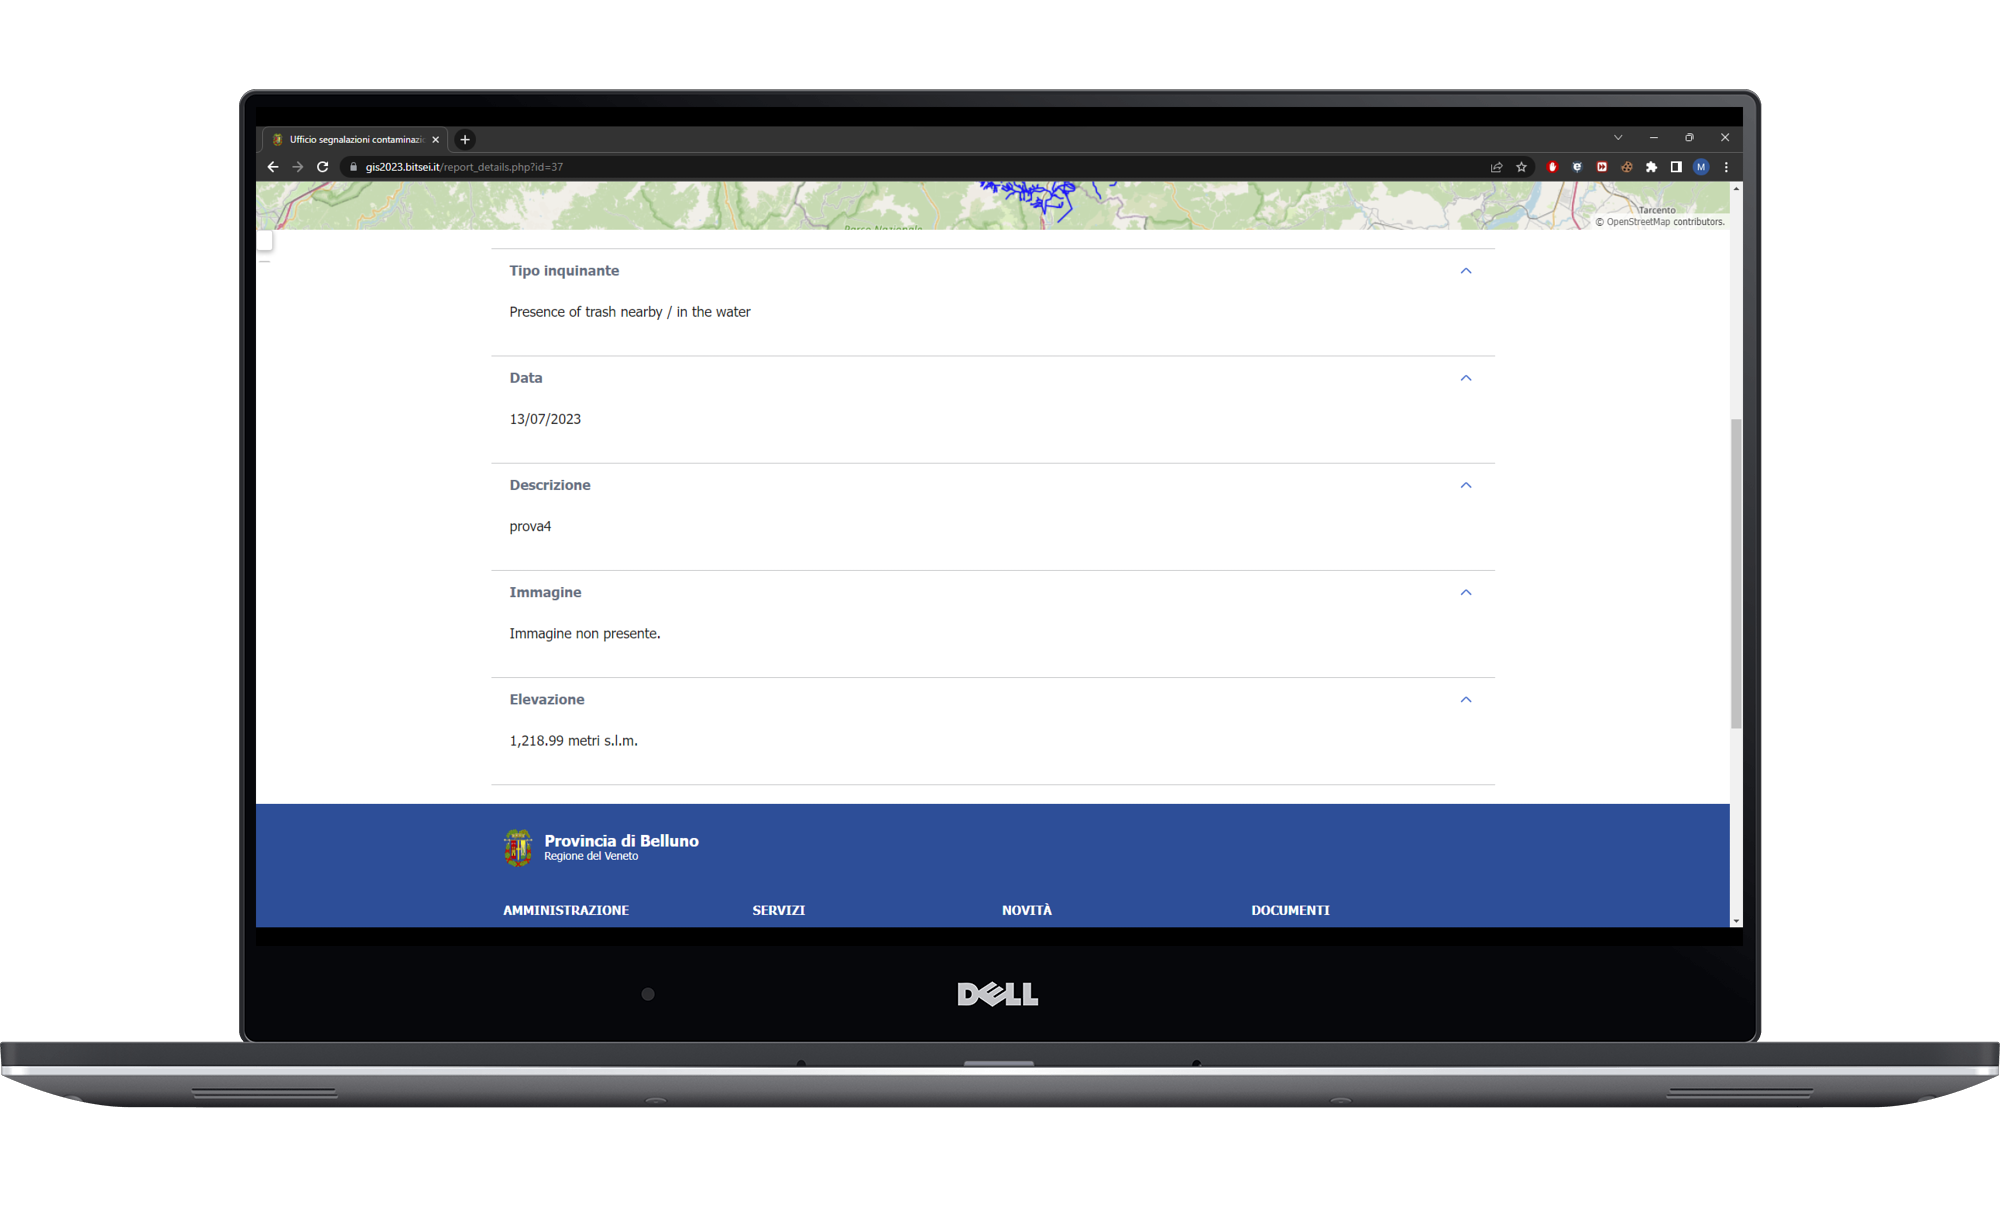
\includegraphics[width=27em]{img/dati_rep.png} \caption{View of report info}  \label{reportView} \end{figure}
    Finally, a summary map that displays the position of all the reports, with the possibility of filtering them by year is available by the button in the home page \textit{Visualizza tutti} [\ref{allPositions}].
    \begin{figure}[H]\centering 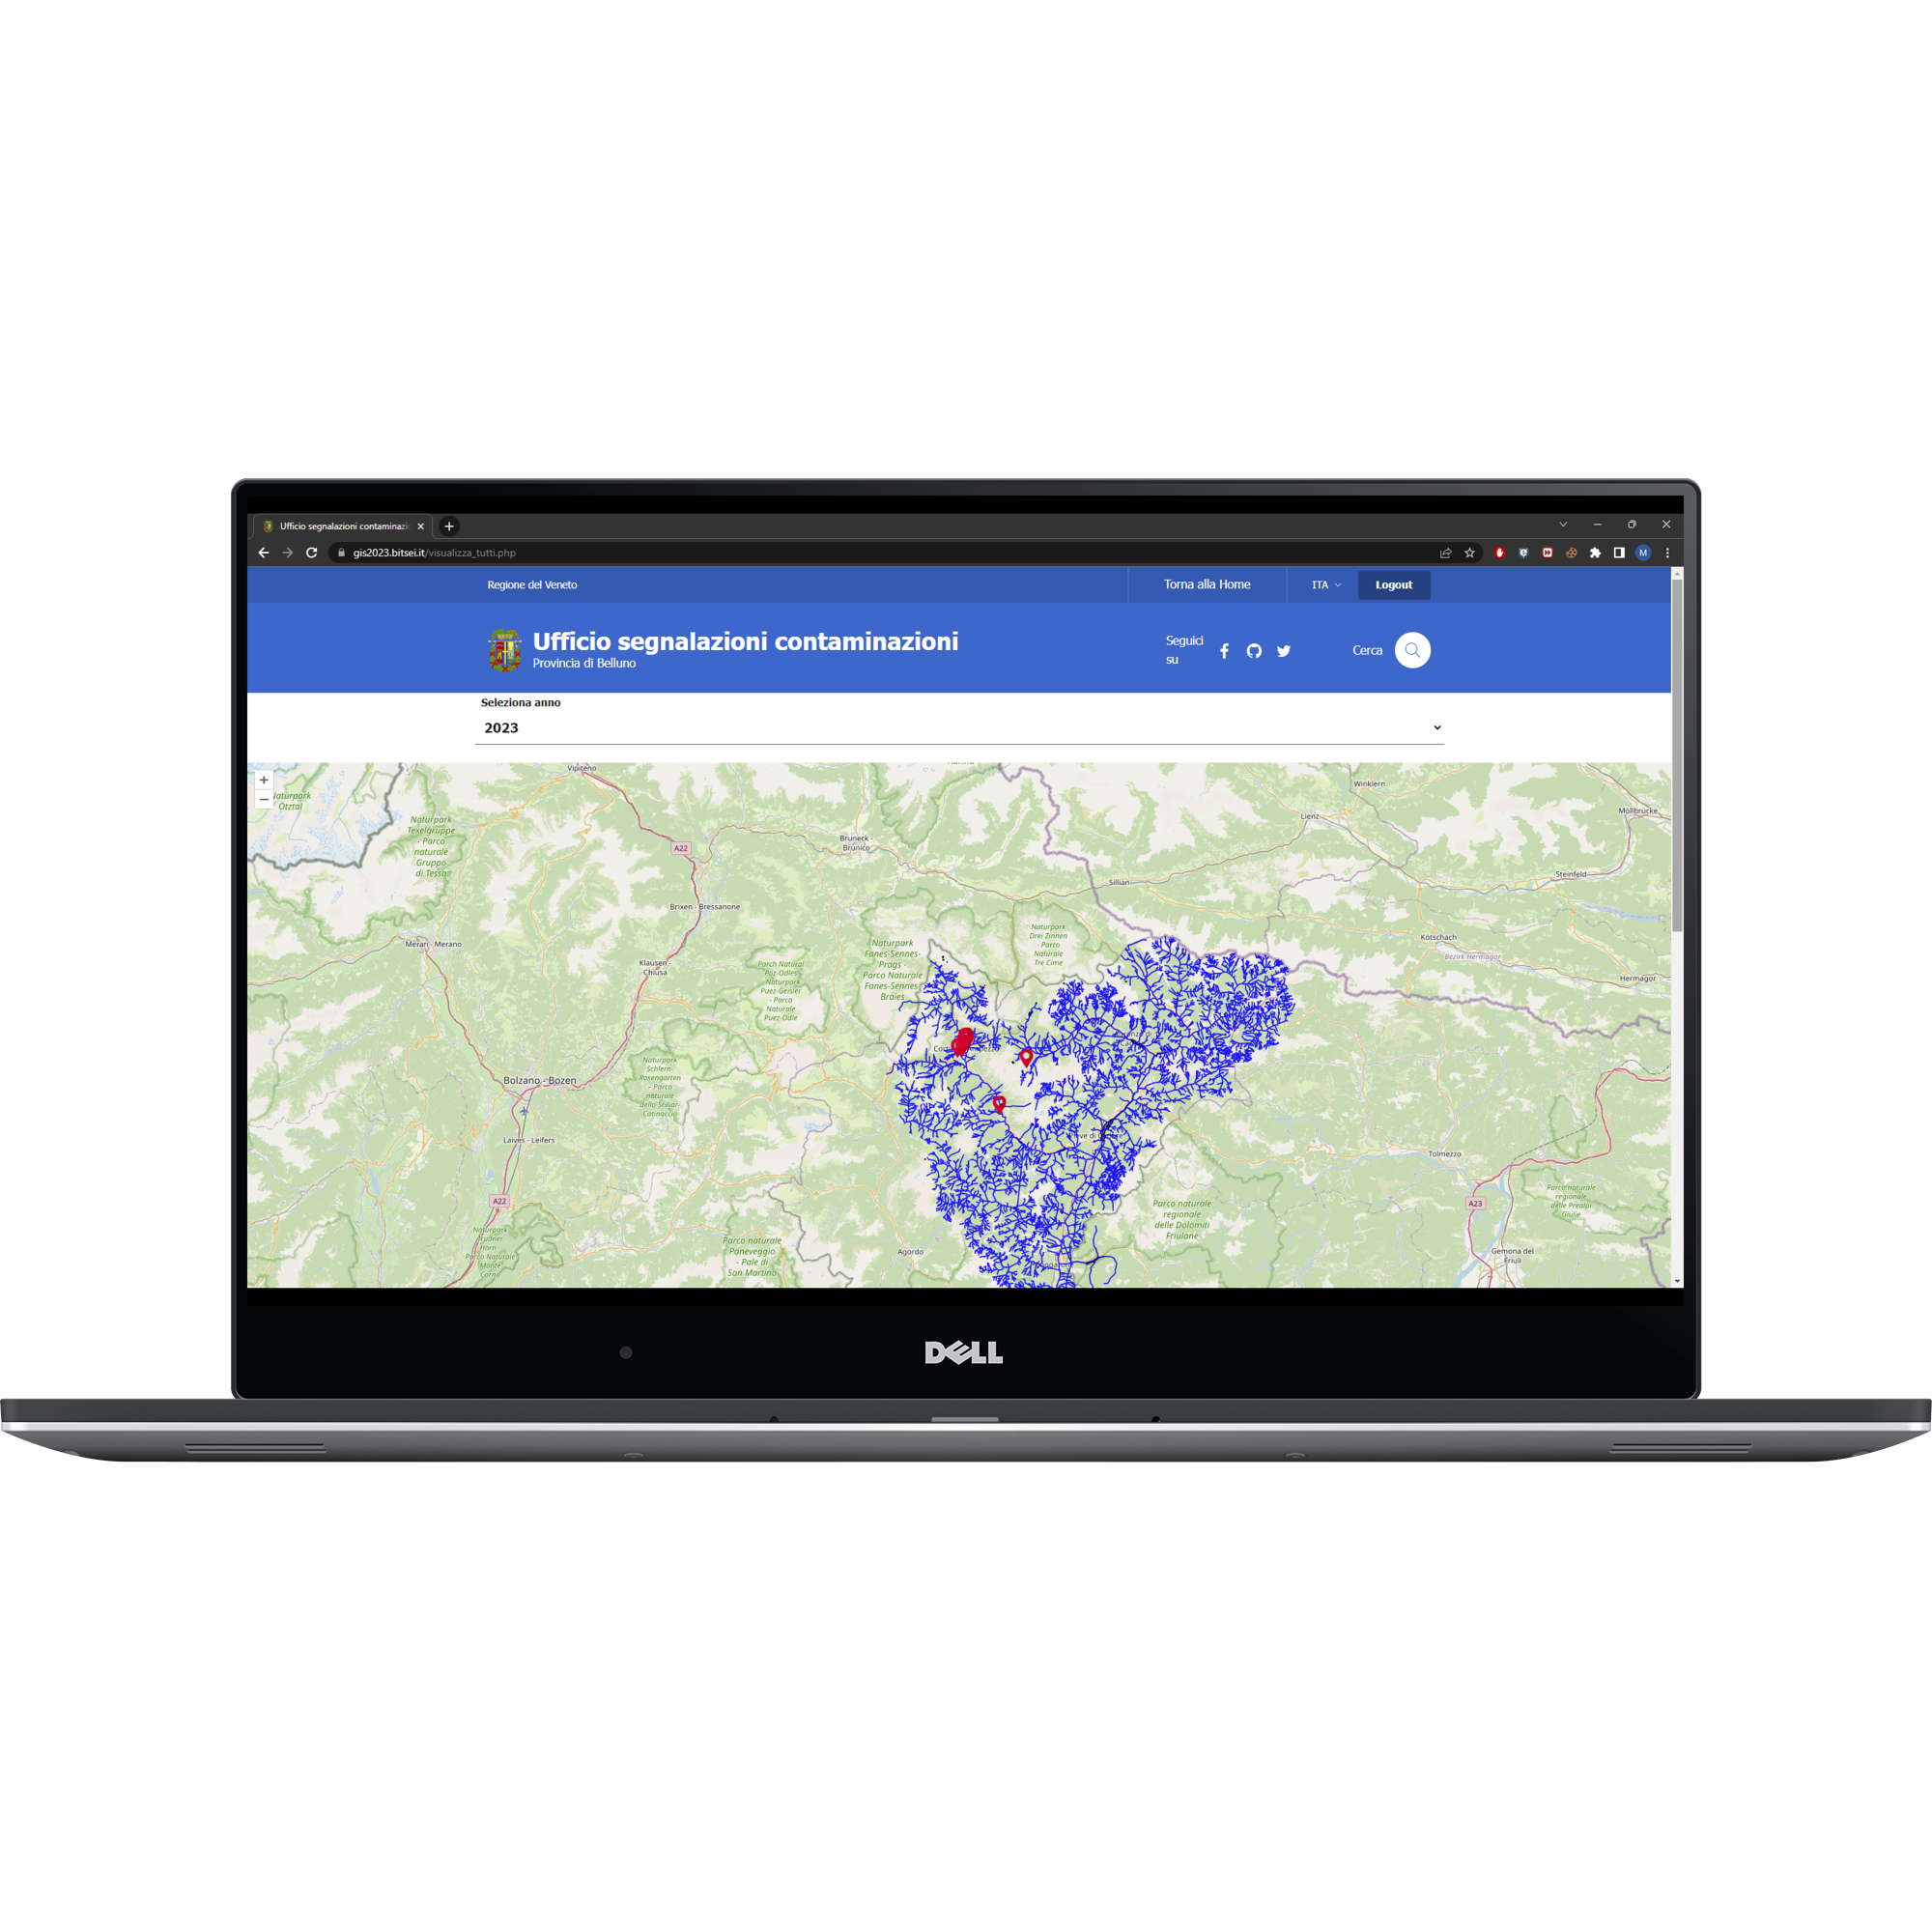
\includegraphics[width=27em]{img/all_reports.png} \caption{View of all report positions} \label{allPositions}\end{figure}
    
\end{itemize}

\subsubsection{OpenJUMP plugin}
The plugin is mainly implemented by 3 classes their functionalities are:

\begin{itemize}
    \item \textit{Plugin.java} Is the main class, it establish the plugin, and it finds the first nearest 3 monitor units and all reports in a 500m range.
    \item \textit{Login.java} By using javaSwing it enables the user for making a login to the database.
    \item \textit{Database.java} It connetes the plugin to the database, it can retrive all the monitor units and report stored.
\end{itemize}

For more tecnical infrmation the projact has a javadoc.

\begin{figure}[H]
    \centering
    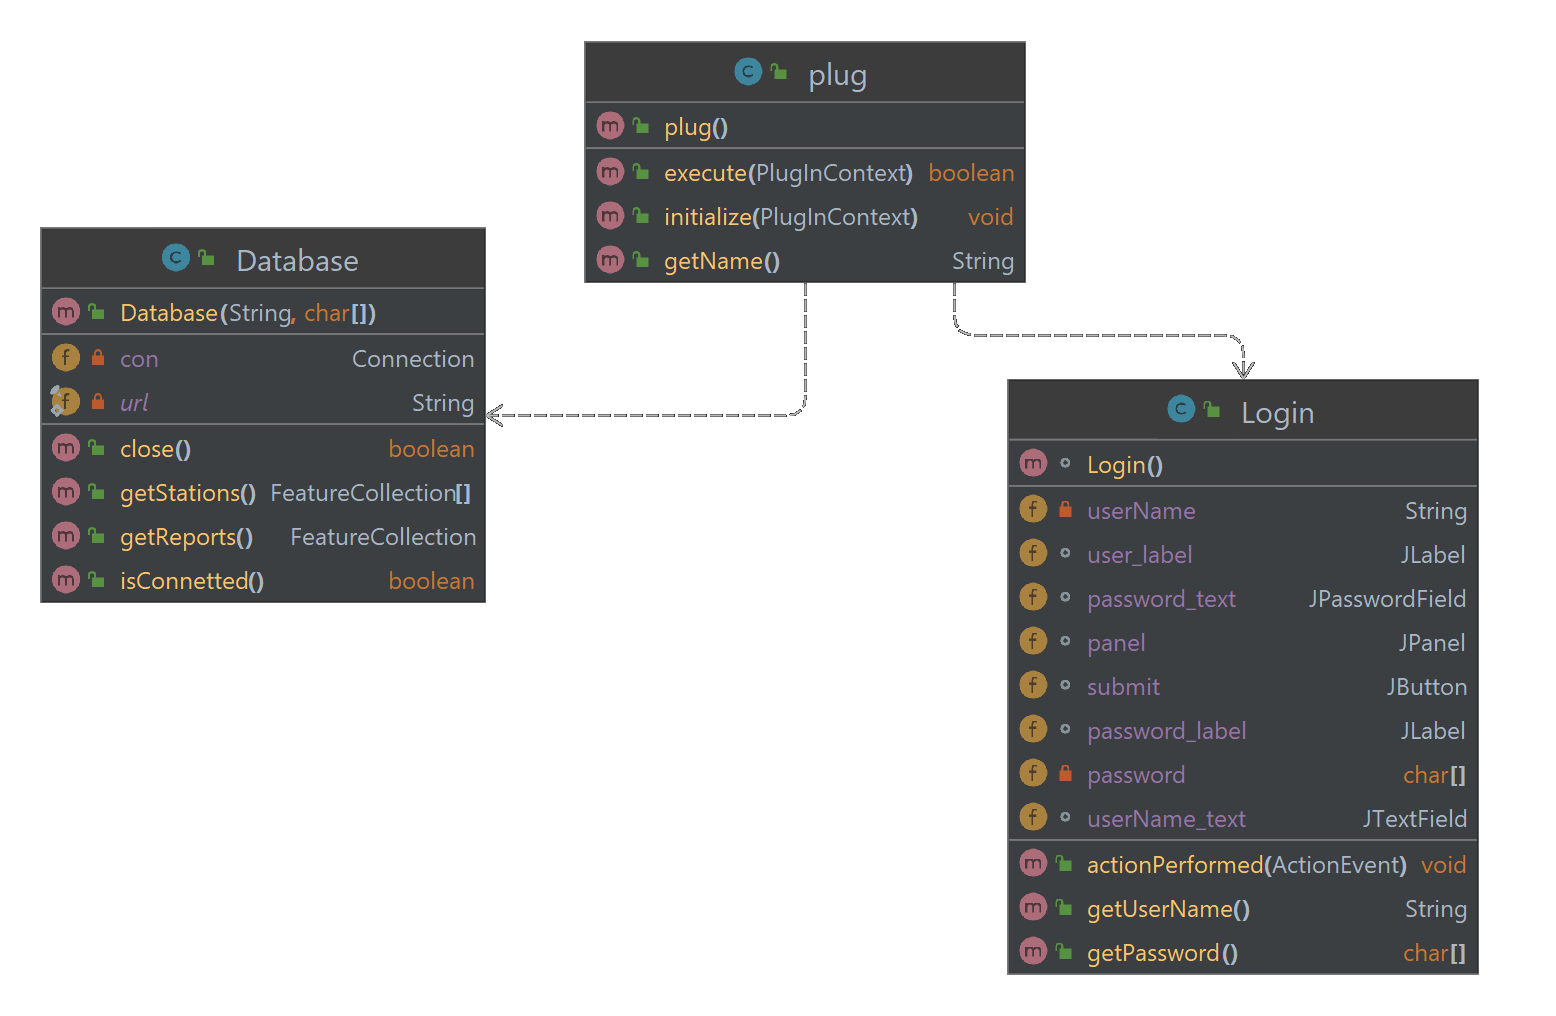
\includegraphics[width=25em]{img/classdiagram.png}
    \caption{UML diagram}
    \label{uml}
\end{figure}
Differently from the webapp, here a specific initial configuration on the user's terminals needs to be setted up.
This kind of initial support is by the way provided by our company and so no tutorial needs to be included in this document. \\
As specified we will use OpenJUMP as GIS desktop software: the open source nature of OpenJUMP grants us the full accessibility of it's interfaces for 2D geometry manipulation.
The Output layers will be located in the "Result" folder. All the relevant data inside the database will be loaded in OpenJUMP so the technician can see all the information about reports and monitor units.
The plugin will work as the following:

\begin{enumerate}
    \item The user will launch the plugin.
    \item The plugin will ask for the credentials for database connection fig:[\ref{optuTorial1}]. 
    \begin{figure}[H]
        \centering
        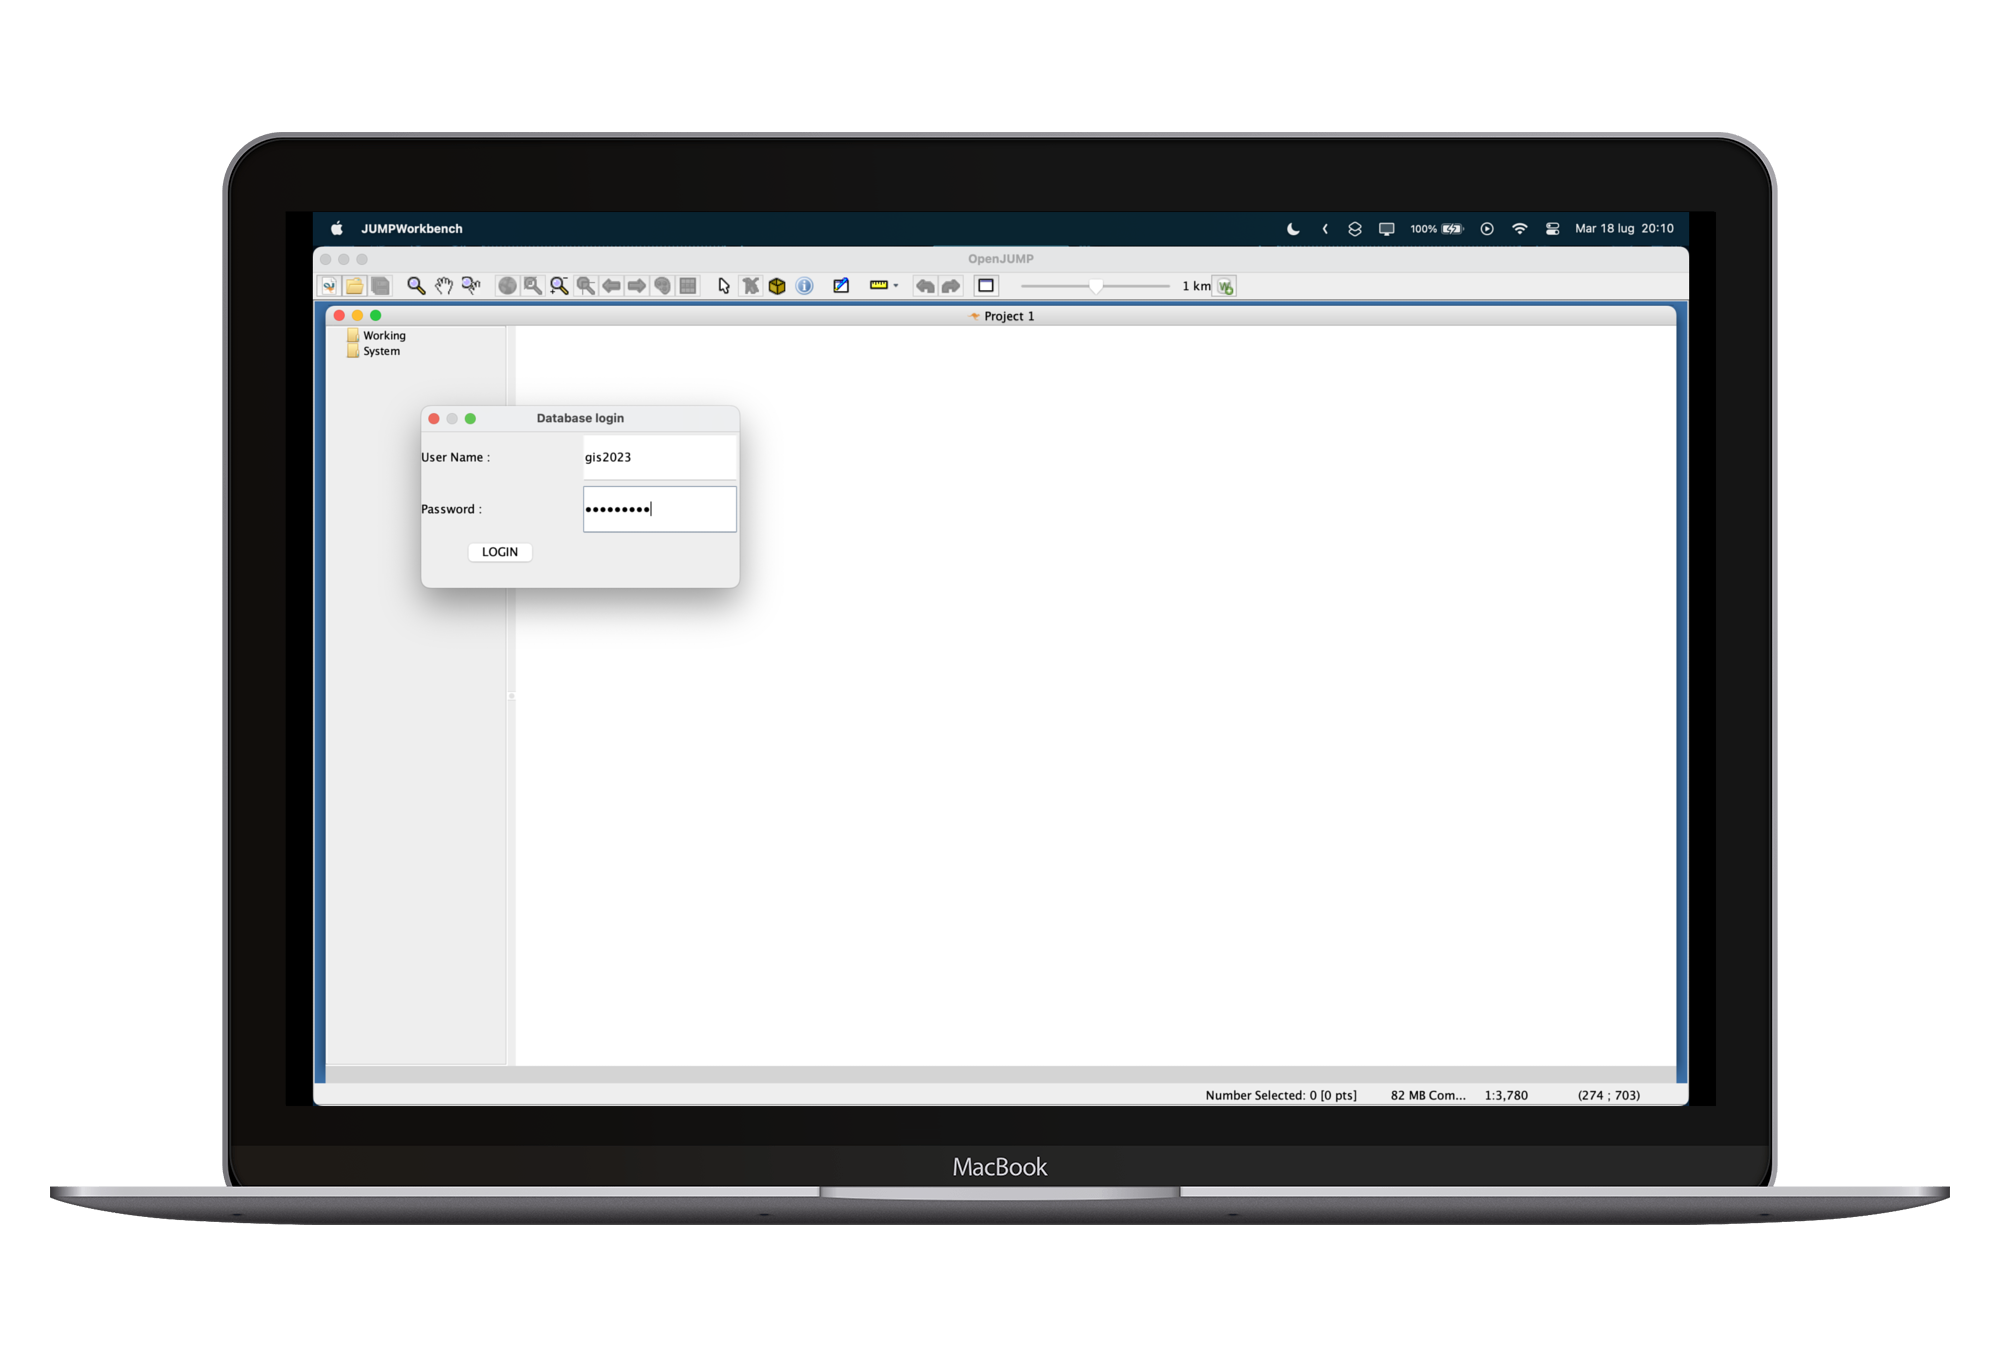
\includegraphics[width=27em]{img/op1.png} \caption{Database login} \label{optuTorial1}
    \end{figure}
    \item The plugin will load the layers of the reports and monitor units.
    \item The user will choose the report to visualize fig:[\ref{optuTorial2}].
    \begin{figure}[H]
        \centering
        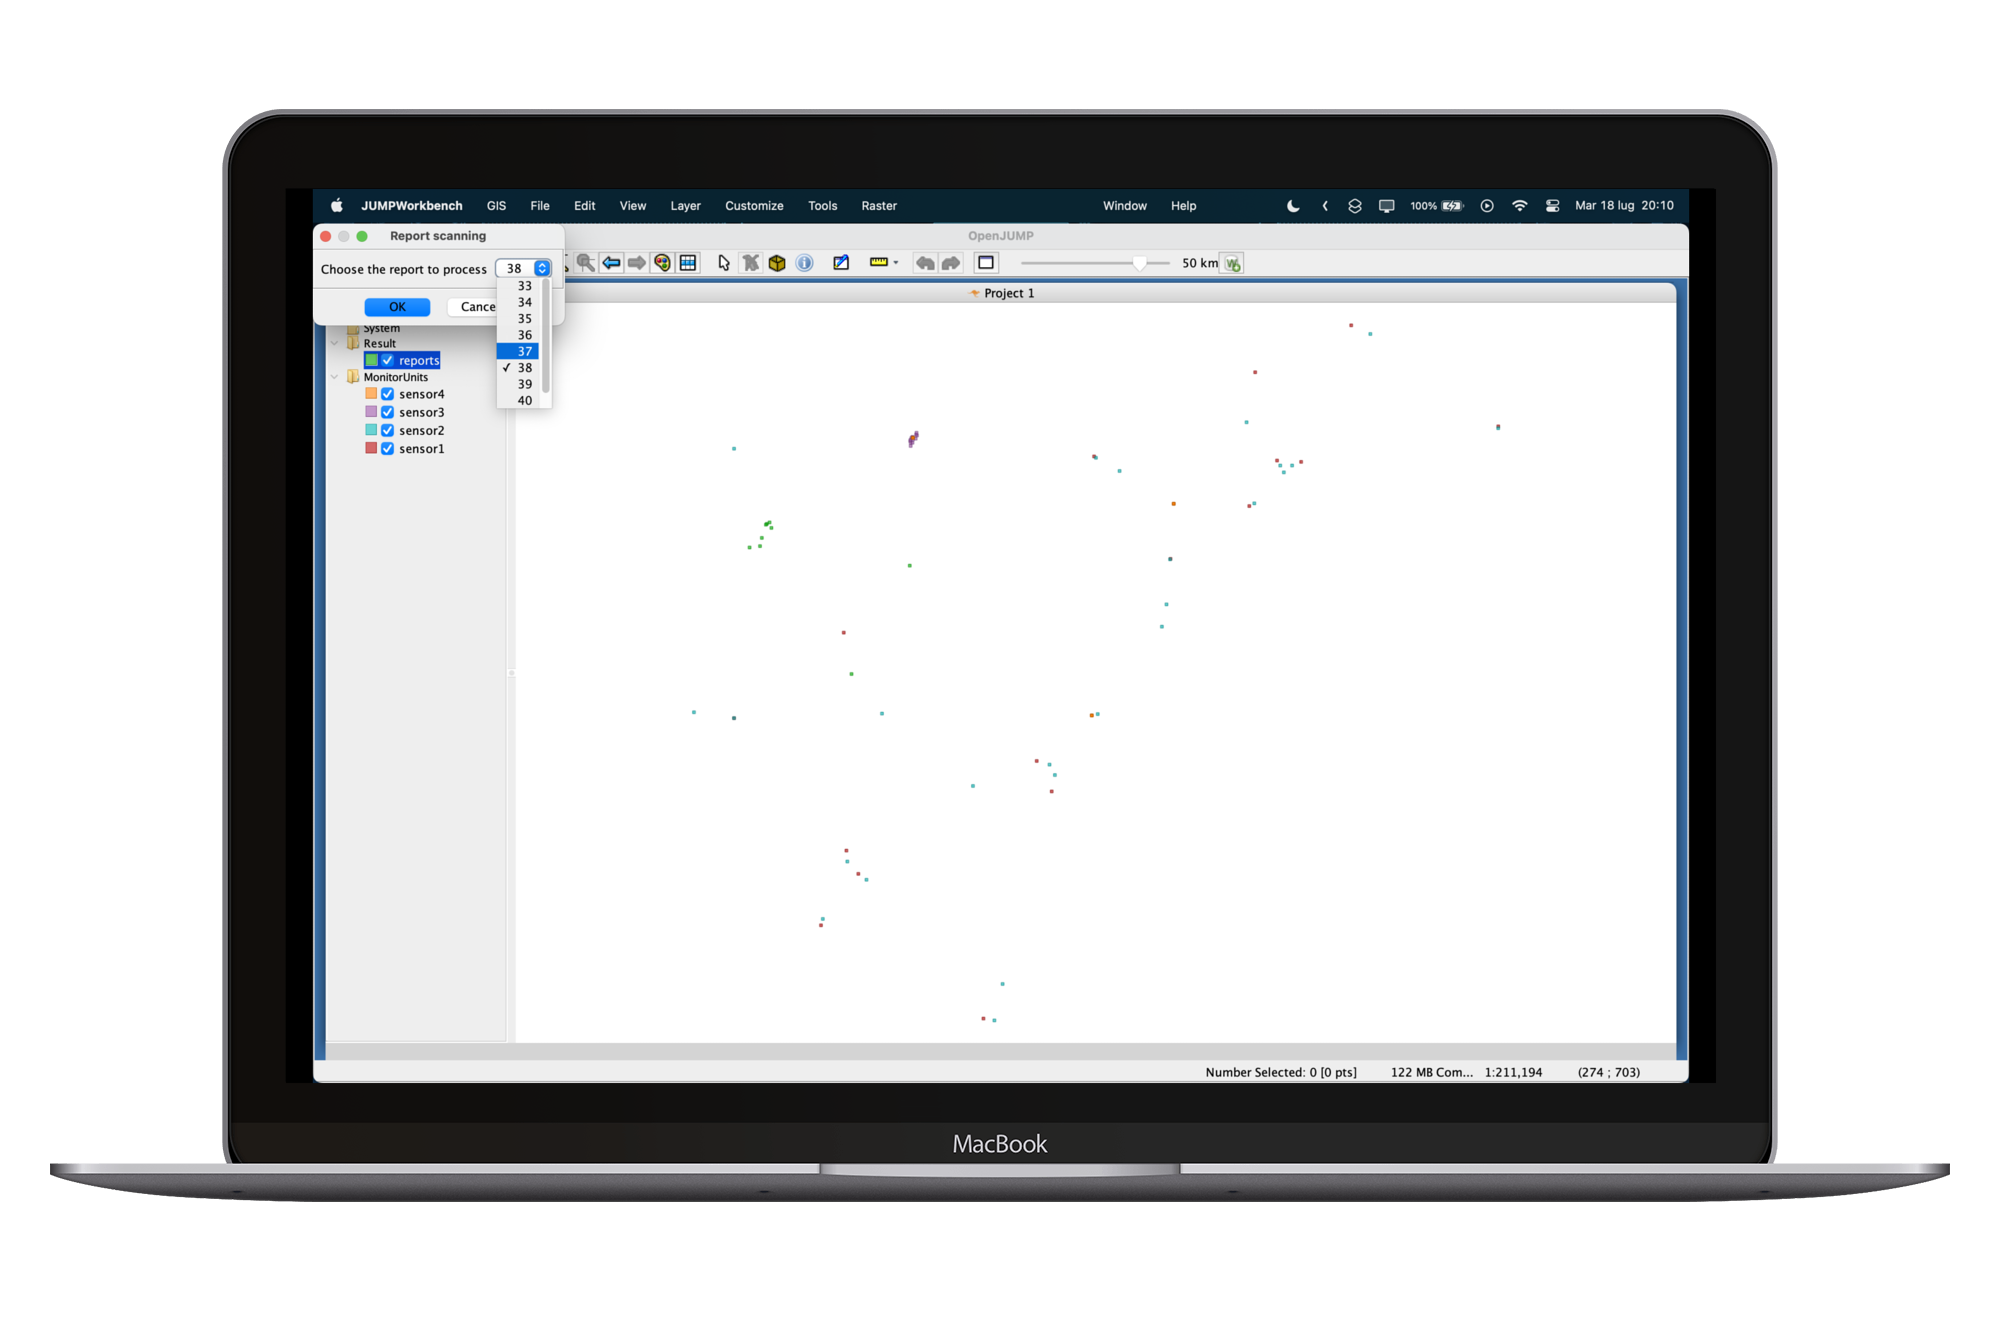
\includegraphics[width=27em]{img/op2.png} \caption{Report selection} \label{optuTorial2}
    \end{figure}

    \item The plugin will find the closest three monitor units to the report position (two upstream one downstream) and they will be linked to the position of the report chosen [\ref{optuTorial3}].
    \begin{figure}[H]
        \centering
        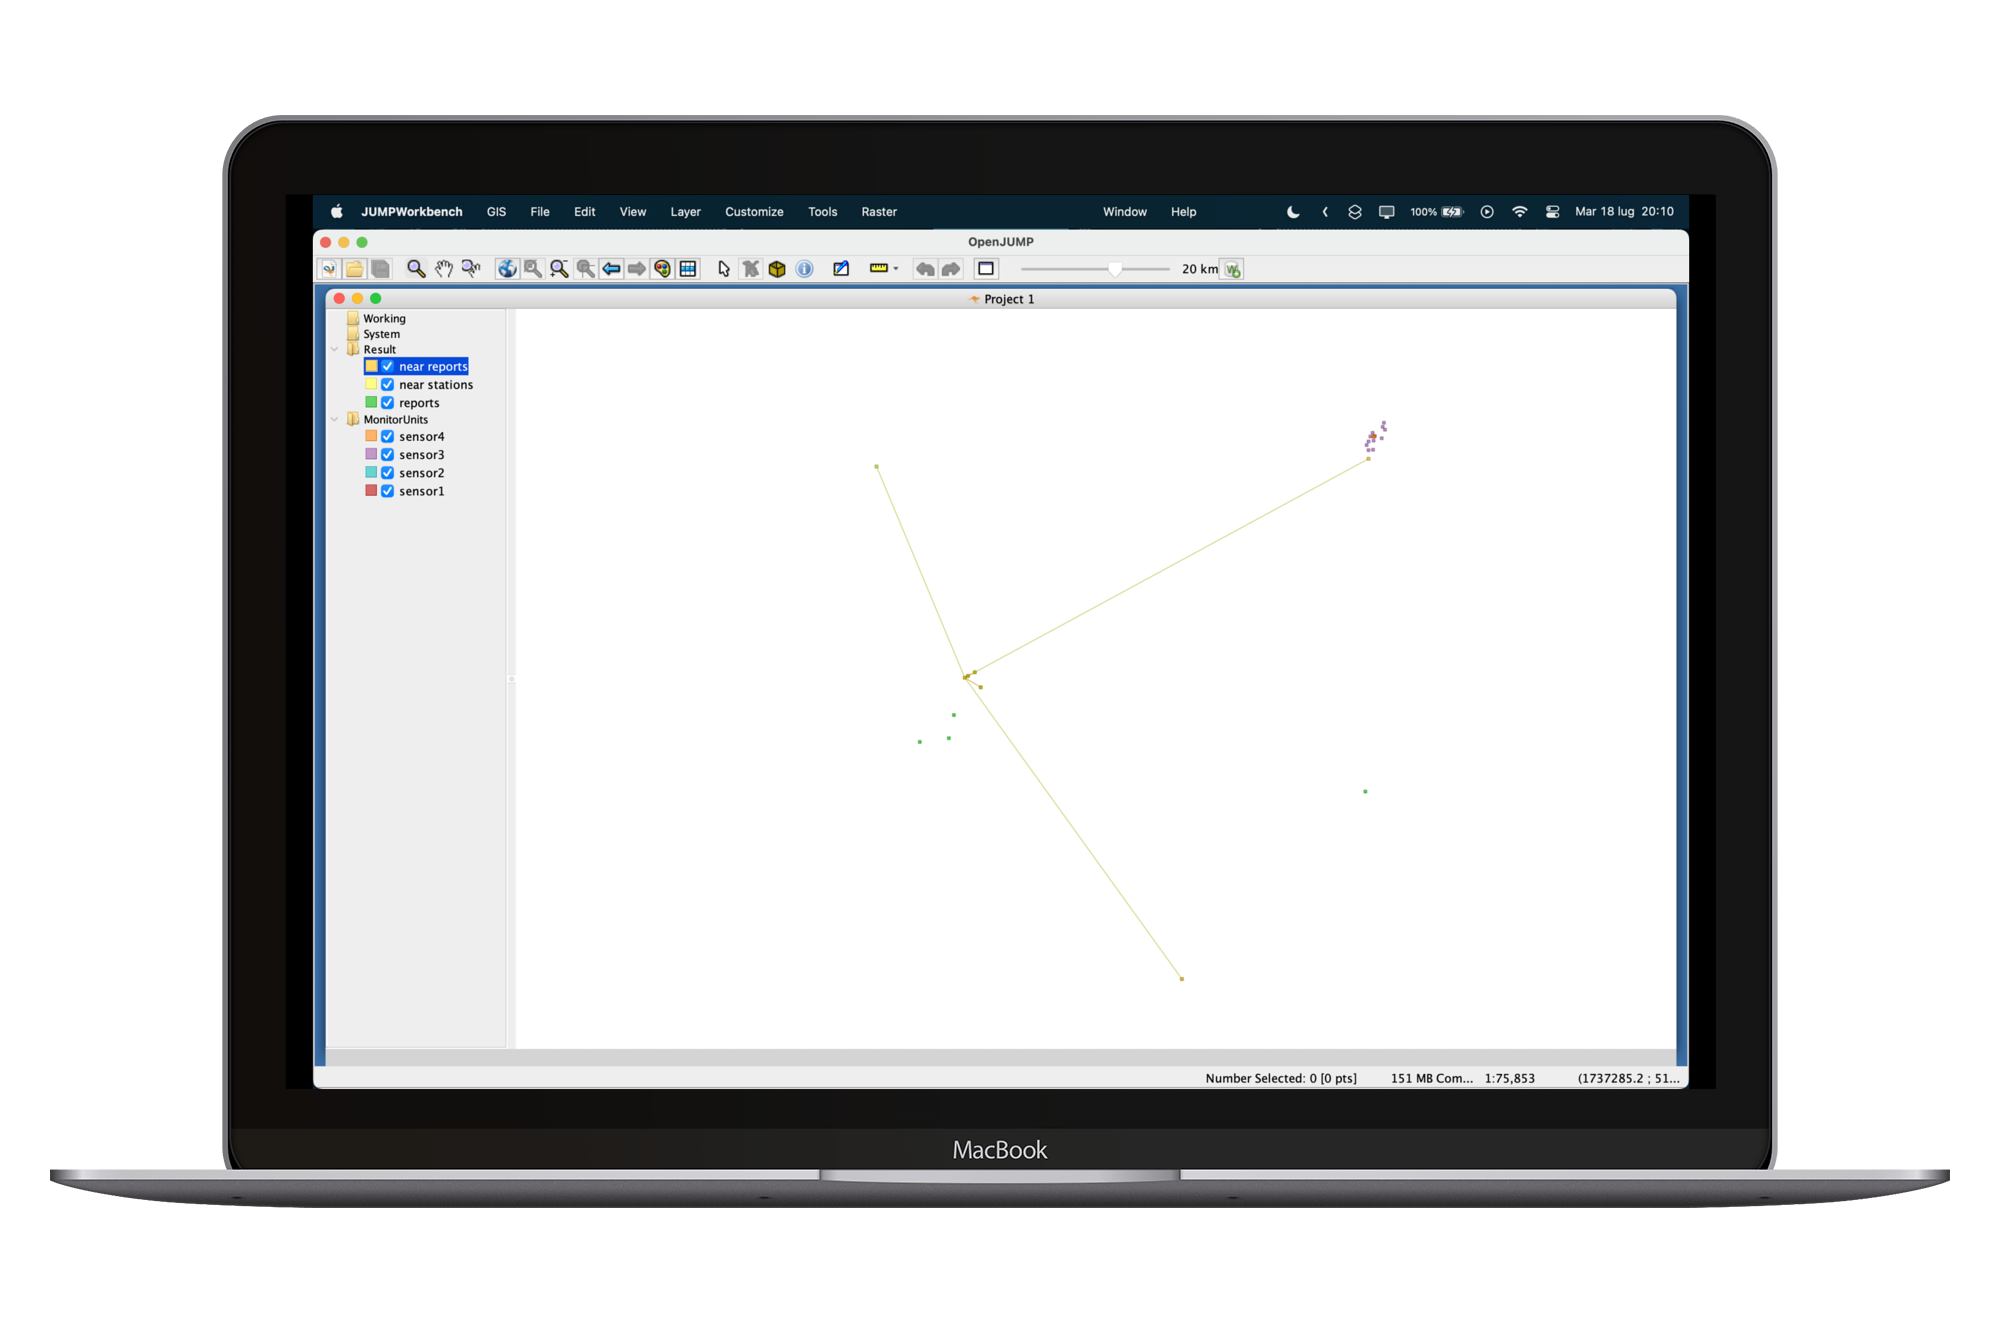
\includegraphics[width=27em]{img/op3.png} \caption{Report connections} \label{optuTorial3}
    \end{figure}

    \item The plugin will find all the reports in a range of 500 meters and they will be linked to the report chosen.
\end{enumerate}



\subsection{Other Features not Implemented}

For the final delibery the project shold have this other features not implemted:

\begin{itemize}
    \item an interface for the 3 technicians that allows them to modify, remove or add the intakes of the various companies, every tecnichian will have it's own account for managing it.
    \item an interface for thetechnicians which allows them to check the maintenance scheduling and indicate when it was done, it can displaye the history of all the maintenance already carried out.
    \item a program that reads the data from the 10 gateways and writes the data to the database.
    \item a danger ranking for the report generated by an AI powered technologies, by using Natural Language Processing (NPL) and Computer Vision techniques the AI will score a ranking in the range 0 to 10, where 10 is very dangerous.
\end{itemize}

\subsection{Database}
\subsubsection{ER Schema}
\begin{figure}[H] \centering 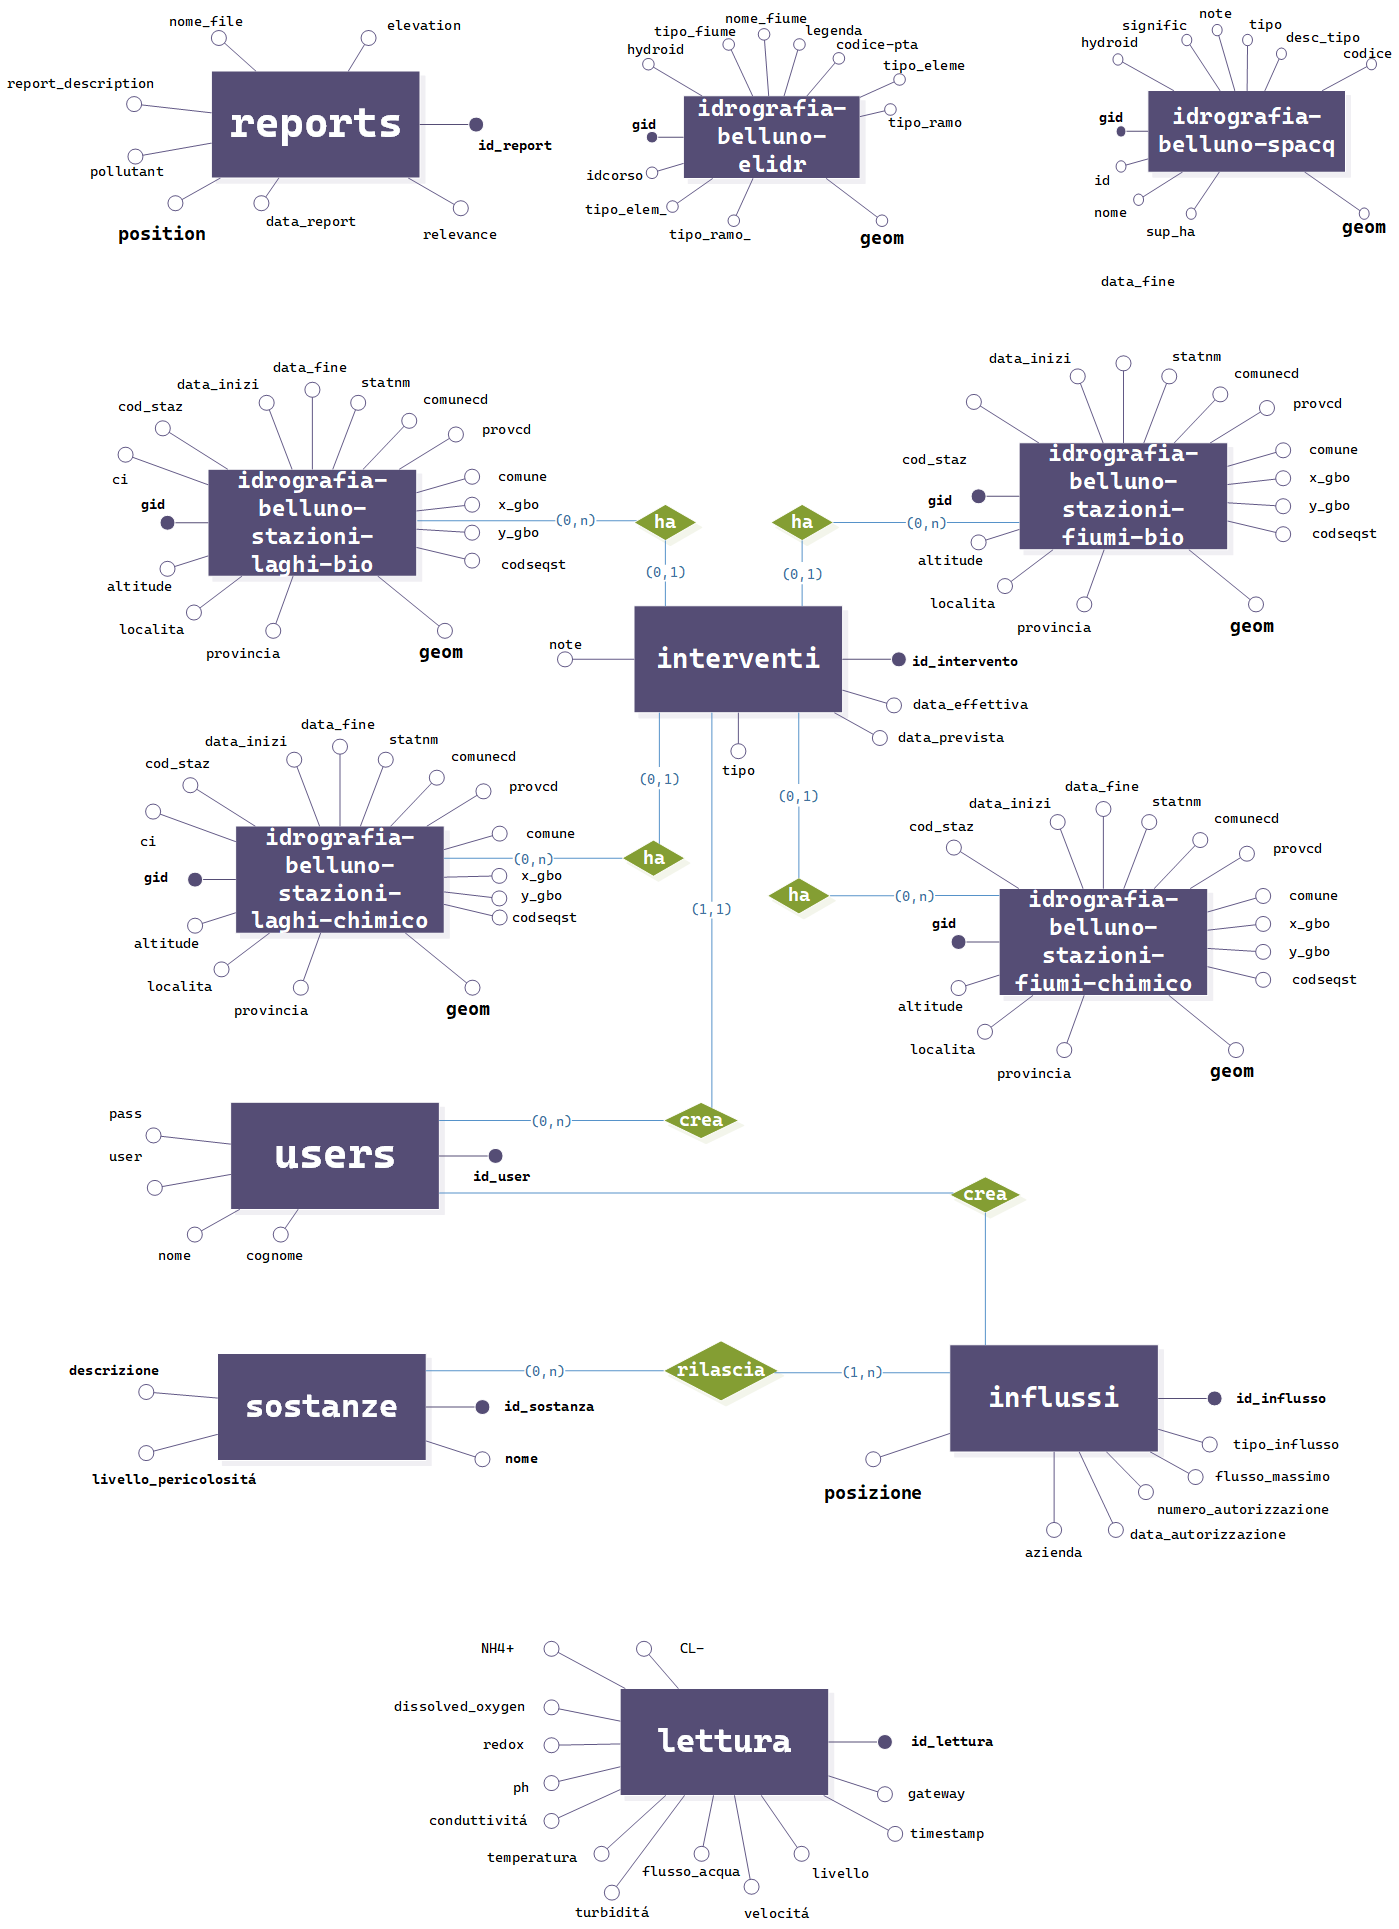
\includegraphics[width=39em]{img/ERSchema.png}  \caption{ER schema} \label{er} \end{figure}

\subsubsection{Description of Entities and Relationships}
As the schema displays Fig[\ref{er}], we can see that six of the entities are related to each shapefile regarding data coming from the Region of Veneto and ARPA Veneto.
For what concerns spatial data representing rivers and lakes, the entities are:
\begin{itemize}
    \item \textit{idrografia-belluno-elidr};
    \item \textit{idrografia-belluno-spacq};
\end{itemize}
The relations that are related to the 4 different typologies of monitoring units instead are:
z\begin{itemize}
    \item \textit{idrografia-belluno-stazioni-laghi-bio};
    \item \textit{idrografia-belluno-stazioni-fiumi-bio};
    \item \textit{idrografia-belluno-stazioni-laghi-chimico};
    \item \textit{idrografia-belluno-stazioni-fiumi-chimico}.
\end{itemize}
As it is visible from the schema, these entities are in relation with the entity \textit{interventi}. This entity represents a maintenance event made by one technincian phisically on a monitoring unit. Due to the limitation of the E-R representation, another constraint need to be exploited: each record in \textit{interventi} has at least and at most one foreign key relation with one record in one of the four stations entities.
An \textit{intervento} is made by one connected \textit{user}: this entity holds data and credentials of each user (technicians and employees) of the provincial office. \\
As a technician user is in charge of making an \textit{intervento}, an employee of the provincial office is in charge (between all) of managing the insertion and the deletion of intakes into rivers and lakes. Intakes are represented by the \textit{influssi} entity, with all the data necessary to represent them. Since a company can release from an intake many different substances, the representation of them in an dedicated entity was necessary: this imply that employee will need to insert, delete or update polluting substances (\textit{sostanze}) separately. \\

Lastly, two important but not relationed entities are in the database:
\begin{itemize}
    \item \textit{reports}: this entity records all the reports made by the citizens. Between all the field, a \textit{relevance} field that as explain before is set to allow future installation of an external software (based on AI technologies) that will be able to assign a relevance score to each report.
    \item \textit{letture}: this entity records the data read from the ten public web gateways that collect the information from the 90 monitoring units. The recording operation of this data is necessary because of the historicization and interrogation requirement.
\end{itemize}

\subsubsection{Data Volumes}
The last two described entities (\textit{reports} and \textit{letture}), differently from the others, can require a lot of disk space on the system server.
A specific analysis of space needed for the reports cannot be exact and neither estimated until we do not have some statistics on the popularity of the system among the citizens: an approach can be to allocate a quite big amount of space initially and to observe the usage in the first months after the installation of the system, so to reduce or increase it. \\
For the \textit{letture} entity is instead possible a more precise estimation: since a separated script in charge of periodically read data from the web gateways and write them on the database will be set up, by knowing the reading frequency (assuming in seconds) of the monitoring units, and assuming an history of one year in the database, the space required from this entity will possibly be: \\
\begin{figure}[H]
    \centering
    \begin{math}
        Space = 60\cdot\frac{86400}{Frequency}\cdot365\cdot90
    \end{math}
    \caption{Approximation of the size of the \textit{readings} table in 1 year.}
    \label{letture_space}
\end{figure}
Where \textit{60} is our estimation in byte of the size of a record, \(\frac{86400}{Frequency}\) is the number of readings per day and \textit{90} is the number of monitoring units [\ref{letture_space}].
   
\subsubsection{Final Considerations}
It is important to keep in mind that even if many relations seem to be missing (i.e. an intake is not linked to the corresponding river nor lake, etc.), a topological database like this can rely on the implicit spatial relations that can be detected in the logic of the application by using topological libraries (i.e. \textit{JTS}) or directly using \textit{PostGIS} functions.
\section{Project guidelines}
\subsection{Deployment plan}
\subsubsection{Scheduling and Timeframes}
   
\begin{figure}[H]
    \centering
    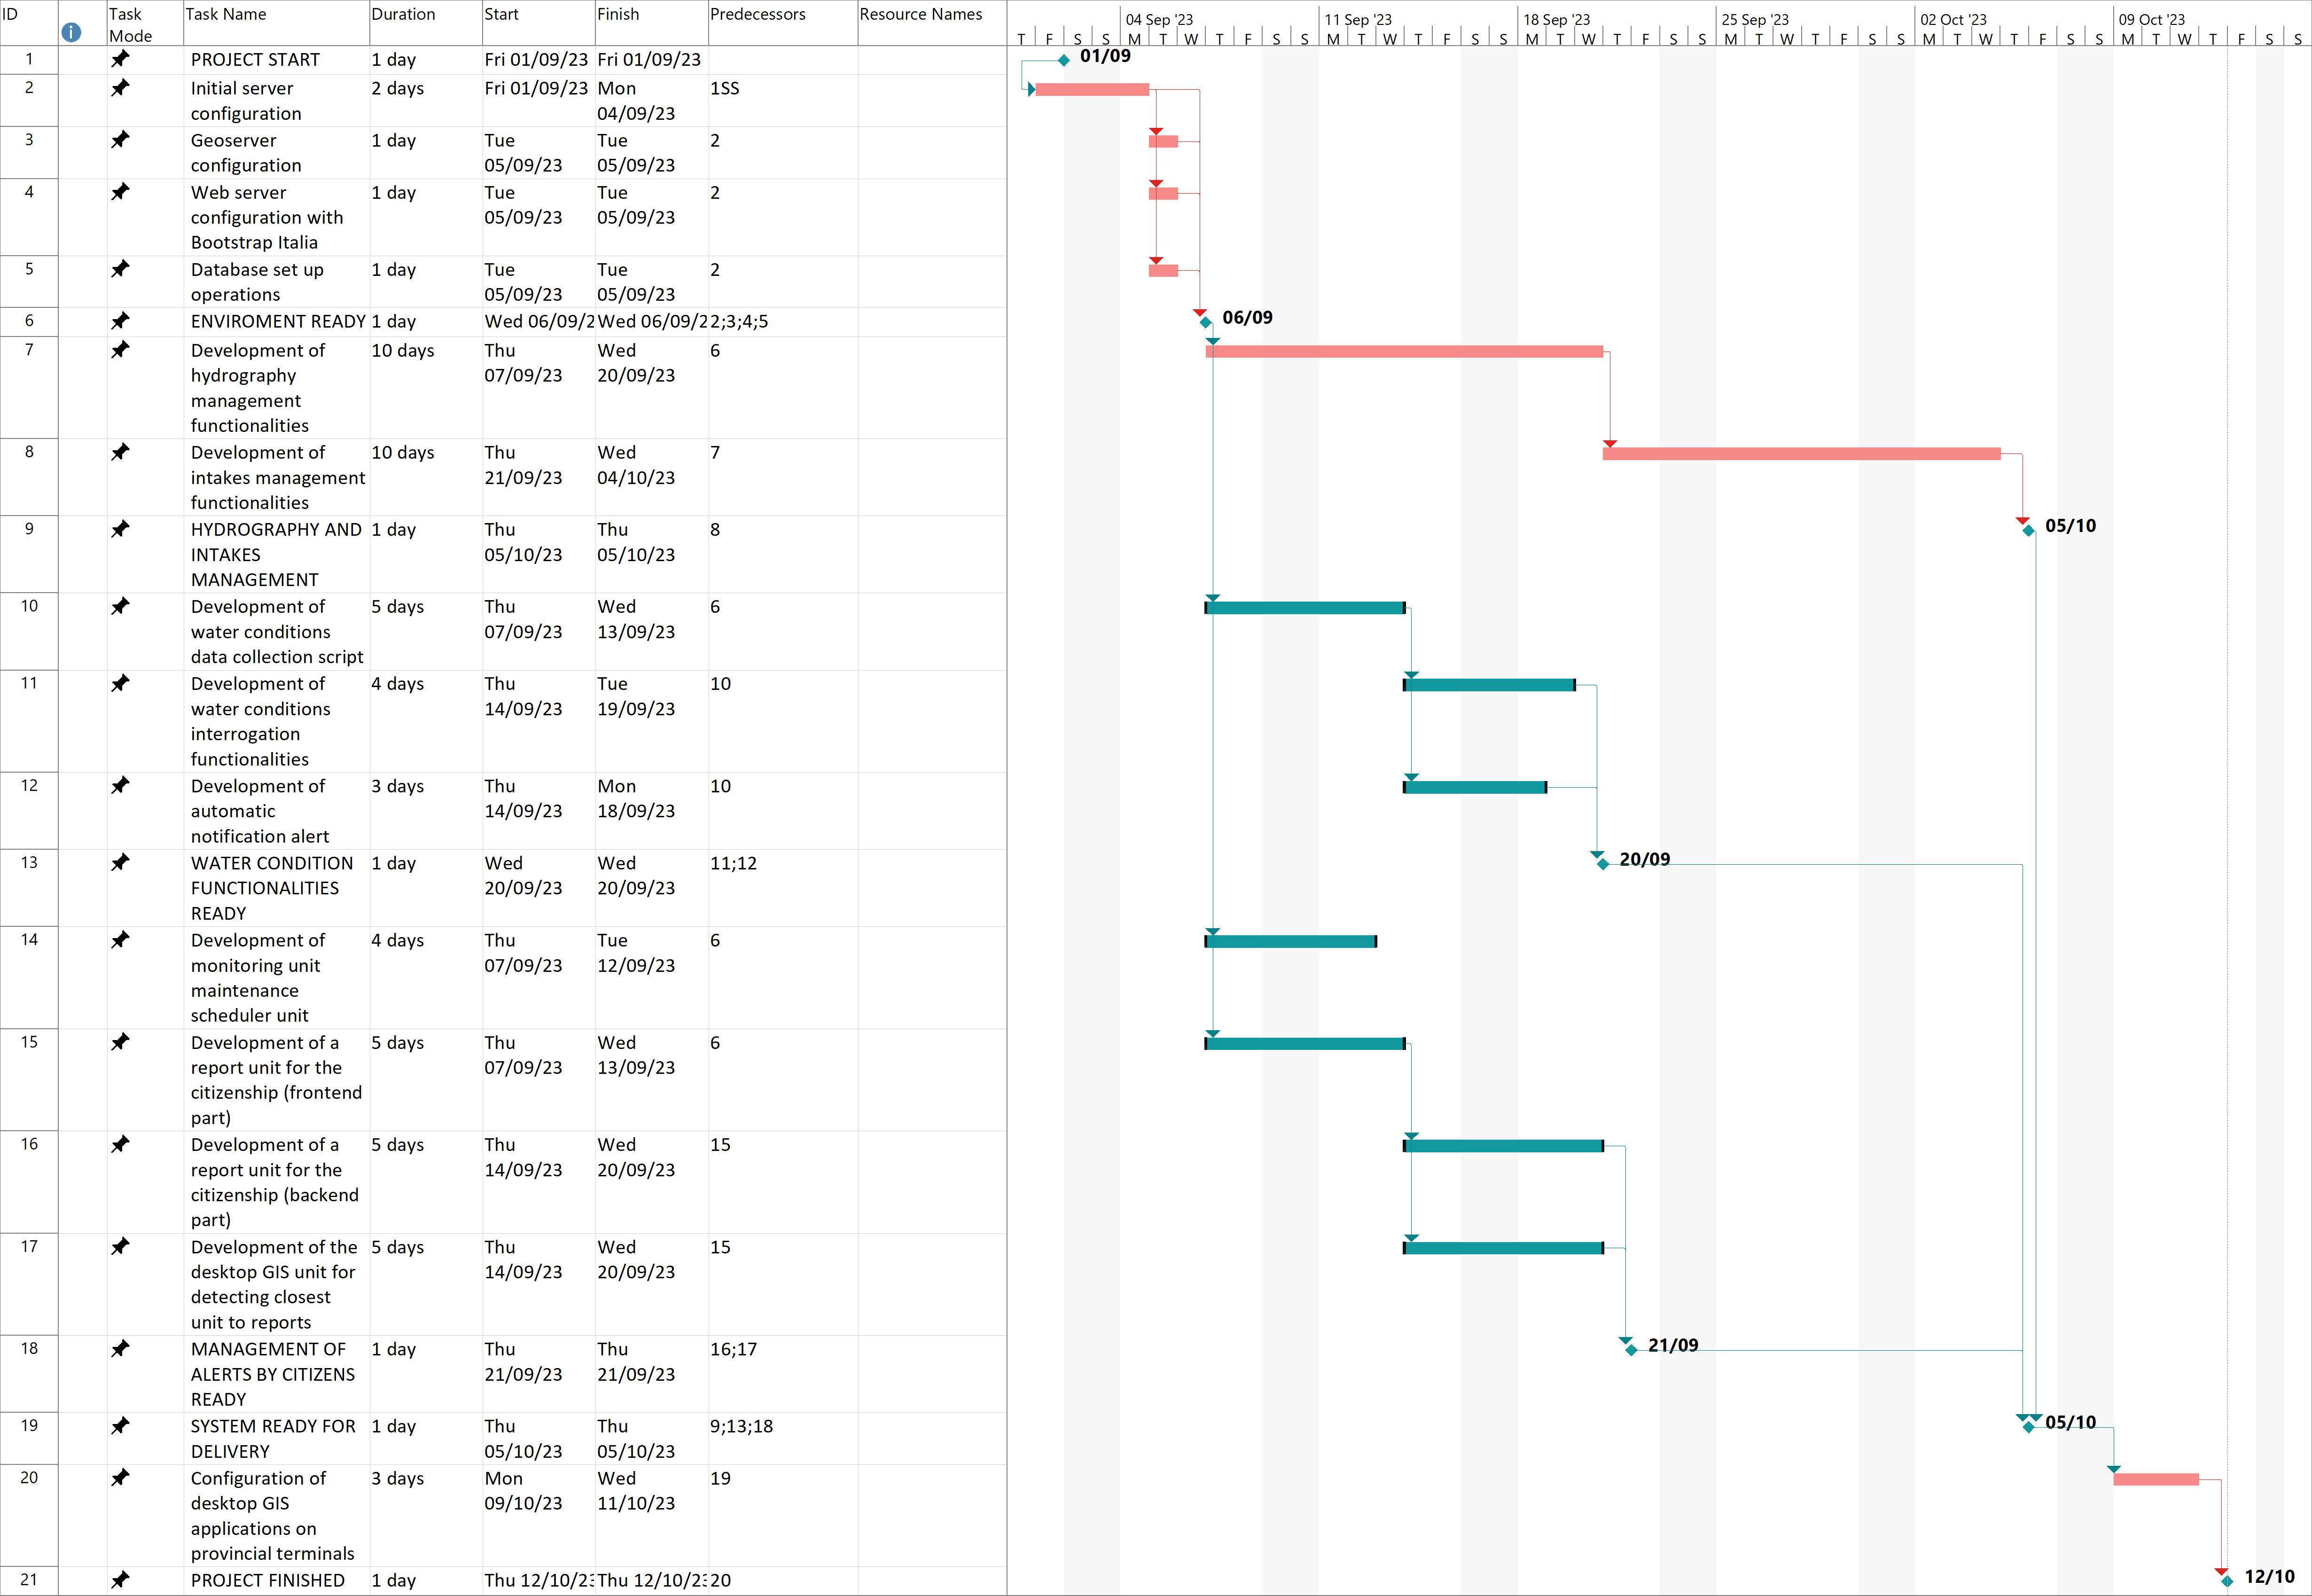
\includegraphics[width=\textwidth]{img/gantt.png}
    \caption{Gantt chart}
    \label{Gantt}
\end{figure}

\subsubsection{Description}
In the Gantt chart are shown all the activities necessary to reach the final goal; the working hypotesis is to start the project by the 1st of September 2023 with the sever configuration procedures and then finish up everything (if no delays happens) by the 12th of October: the whole execution then should take around one month and a half.
This hypotesis does not take care of the number of working resources (software engineers or programmers) available for the execution, that can led to a more constrained execution due to many parallelized activities. \\
Activities coloured in pink represents the \textit{critical path}, that are the ones in which a delay can led to a delay of the whole project.

\subsubsection{Deliverables}
From the Gantt chart is visible that three main milestone are present in the timeline of the project: these coincides with three different \textit{deliverables}, that are three tangible and atomically usable parts of the system.\\
In particular:
\begin{itemize}
    \item \textbf{05/10}: this milestone coincides with the delivery of the hydrography and intakes management functionalities. Theoretically, from this date the provincial employees can start to use and to test this subpart of the system;
    \item \textbf{20/09}: this milestone coincides with the delivery of the automatic data reading subsystem from the web gateways and the email alert system. Theoretically, from this date the provincial employees can start to use and to test this subpart of the system;
    \item \textbf{21/09}: this milestone coincides with the delivery of the reporting subsystem for the citizenship and its backend and desktop management functionalities. Theoretically, from this date the provincial employees can start to use and to test this subpart of the system.
\end{itemize}

\pagebreak
\subsection{Risk management}
Many activities can be conducted to study risks in a project. One possible approach can be to conduct a \textit{FMEA} analysis, but the size of the actual project is not so big to justify such an extensive analysis. \\
A better approach for the actual project has been found in filling a risk register.

\subsubsection{Risk matrix}
To evaluate the level of a risk (in a scale of three levels, \textit{low}, \textit{medium} and \textit{high}) we can use the risk matrix that is defined as follows:
\begin{table}[H]
    \centering
    \begin{tabular}{|cc|c|c|c|}
    \hline
    \multicolumn{2}{|l|}{\textbf{IMPACT}}                      & Low    & Medium & High   \\ \hline
    \multicolumn{1}{|l|}{\multirow{3}{*}{\rotatebox{90}{\textbf{PROB.}}}} & High   & \cellcolor{orange!25}Medium & \cellcolor{red!25}High & \cellcolor{red!25}High   \\ \cline{2-5} 
    \multicolumn{1}{|l|}{}                   & Medium & \cellcolor{green!25}Low    & \cellcolor{orange!25}Medium & \cellcolor{red!25}High   \\ \cline{2-5} 
    \multicolumn{1}{|l|}{}                   & Low    & \cellcolor{green!25}Low    & \cellcolor{green!25}Low    & \cellcolor{orange!25}Medium \\ \hline
    \end{tabular}
    \caption{Risk Matrix}
    \label{matrix}
\end{table}

\subsubsection{Risk register}
\begin{table}[H]
    \centering
    \begin{tabularx}{\columnwidth}{|X|X|X|c|c|c|c|}
    \hline
    \textbf{DESCR.} & \textbf{CAUSE} & \textbf{DAMAGE} & \textbf{PROB.} & \textbf{IMPACT} & \textbf{LEVEL} & \textbf{ACTION} \\ \hline
    Data breach & Malicious intrusion with the purpose of steal data & Sensible data exiting from the system & \cellcolor{green!25}L & \cellcolor{orange!25}M & \cellcolor{green!25}L & Mitigate \\ \hline
    Denial of service & Malicious will of attackers of blocking the system & Unavailability of the system & \cellcolor{green!25}L & \cellcolor{red!25}H & \cellcolor{orange!25}M & Mitigate \\ \hline
    Monitoring unit malfunctioning & Broken sensor (not detected) that returns uncorrect data & Uncorrect alerts sent by mail & \cellcolor{green!25}L & \cellcolor{red!25}H & \cellcolor{orange!25}M & Transfer \\ \hline
    Impossibility of data acquisition & Unit readings not returned due to mobile network malfunctions & Missing pollutants monitoring in a certain unit of time & \cellcolor{green!25}L & \cellcolor{red!25}H & \cellcolor{orange!25}M & Transfer \\ \hline
    Fake reporting & Malicious will from citizens to report unreal alterations & Untrustable data & \cellcolor{orange!25}M & \cellcolor{orange!25}M & \cellcolor{orange!25}M & Accept \\ \hline
    \end{tabularx}
    \caption{Risk register}
    \label{register}
\end{table}

\pagebreak
\subsection{Benefits evaluation}
\subsubsection{Benefits identification}
By analyzing the system's functionalities and capabilities, we identify the following benefits:
\begin{itemize}
    \item Fast water pollution detection and circumscription: in case of polluting events, by the alert system is possible to isolate the pollutants quickly, contacting the authorities and avoiding reclaim activities;
    \item Transparent governance: the dedicated portal for water quality analysis results and the citizen reporting system will promote transparency in governance. Citizens will actively participate in the supervision of the province's water heritage by reporting incidents and alterations, fostering a sense of responsibility and engagement in environmental protection;
    \item Data-driven decision making: The system's capabilities for querying and visualizing data will provide valuable insights for informed decision-making. By analyzing historical data and monitoring trends, the province can proactively address water-related challenges, implement preventive measures, and optimize resource allocation;
    \item Improved efficiency and data accessibility: with the implementation of a user-friendly WebGIS application and advanced querying capabilities, accessing and retrieving hydrography data will become more efficient and streamlined. Technical offices and authorized personnel will have real-time access to essential information, reducing response times for critical interventions;
    \item Compliance with standards and regulations: through adherence to relevant hydrography management standards and regulations, the system will ensure that the province's water management practices align with national and international guidelines. This compliance will enhance the province's reputation and bolster its commitment to responsible water resource management.
\end{itemize}

\subsubsection{Economic quantification of the benefits}
An exact estimation of the benefits when talking about the management of a such eterogeneus natural environment that can be harmed by pollutants its hard to discuss. \\
What is important to notice, in our opinion, is that among all the benefits identified above, the first one is the most important; to reclaim a polluted river, or worstly, a lake, can be an activity extremely costly (millions of euros), and such an activity can be even not practicable in certain cases. The possibility of avoiding an heavy and irreversible pollution event of an enviroment in an \textit{UNESCO Heritage} in our opinion has no price. \\
That said, other "minor" (with respect to the previous) benefits can be estimated:
\begin{itemize}
    \item Transparent governance: the possibility of having active citizens can avoid the necessity of technicians going around the province to sketch possible polluting events, avoiding a \textit{RAL} of around \textit{25.000€ - 30.000€} per technician;
    \item Improved efficiency and data accessibility: the easyness of data availability for provincial employees can avoid many working hours of browsing just to find the correct data necessary;
    \item Compliance with standards and regulations: this benefit benefits in different ways: for example, the compliance with standards will allow the province to integrate further functionalities based on future available data. Moreover, this will allow the province to sell data acquired from reports and intake management to other public or private bodies.
\end{itemize}

\subsection{Cost evaluation}
\subsubsection{Project costs}
We summarized the costs related to the starting project considering five different categories of costs:
\begin{table}[H]
    \begin{tabularx}{\columnwidth}{|X|c|c|c|}
    \hline
    \textbf{ACTIVITY} & \textbf{UNIT COST} & \textbf{QUANTITY} & \textbf{TOTAL} \\ \hline
    VIRTUAL SERVER ACTIVATION & 250€ & 1 & 250€ \\ \hline
    SERVER CONFIGURATION & 40€ & 40h & 1.600€ \\ \hline
    WEB DEVELOPING & 55€ & 320h & 17.600€ \\ \hline
    DESKTOP PLUGINS DEVELOPMENT & 45€ & 40h & 1.800€ \\ \hline
    DATA READER SCRIPT FROM MONITORING UNITS & 45€ & 64h & 2.880€ \\ \hline
    CONFIGURATION OF DESKTOP GIS ENVIRONMENT & 40€ & 24h & 960€ \\ \hline
    \noalign{\hrule height 2pt}
    \multicolumn{3}{|l|}{\textbf{TOTAL}} & \textbf{25.090€} \\ \hline
    \end{tabularx}
    \caption{Project cost}
    \label{projectCost}
\end{table}

\subsubsection{Running costs}
We estimated the costs related to the maintenance of the system (based on an annual scale) considering two categories of costs:
\begin{table}[H]
    \begin{tabularx}{\columnwidth}{|X|c|c|c|}
    \hline
    \textbf{ACTIVITY} & \textbf{UNIT COST} & \textbf{QUANTITY} & \textbf{TOTAL} \\ \hline
    VIRTUAL SERVER RENEWAL & 250€ & 1 & 250€ \\ \hline
    ASSISTANCE PLAN & 40€ & 20h/month & 9.600€ \\ \hline
    \noalign{\hrule height 2pt}
    \multicolumn{3}{|l|}{\textbf{TOTAL}} & \textbf{9.850€} \\ \hline
    \end{tabularx}
    \caption{Running cost}
    \label{runningCost}
\end{table}

\end{document}